\documentclass[a4paper]{article}

\usepackage[pdftex,
  hidelinks,
  pdfauthor={Dexter Chua},
  pdfsubject={Cambridge Maths Notes: Part IA - Vector Calculus},
  pdftitle={Part IA - Vector Calculus},
pdfkeywords={Cambridge Mathematics Maths Math IA Lent Vector Calculus}]{hyperref}

\title{Part IA - Vector Calculus}
\author{Lectured by B. Allanach}
\date{Lent 2015}

% Imports
\ifx \nextra \undefined
  \usepackage[pdftex,
    hidelinks,
    pdfauthor={Dexter Chua},
    pdfsubject={Cambridge Maths Notes: Part \npart\ - \ncourse},
    pdftitle={Part \npart\ - \ncourse},
  pdfkeywords={Cambridge Mathematics Maths Math \npart\ \nterm\ \nyear\ \ncourse}]{hyperref}
  \title{Part \npart\ - \ncourse}
\else
  \usepackage[pdftex,
    hidelinks,
    pdfauthor={Dexter Chua},
    pdfsubject={Cambridge Maths Notes: Part \npart\ - \ncourse\ (\nextra)},
    pdftitle={Part \npart\ - \ncourse\ (\nextra)},
  pdfkeywords={Cambridge Mathematics Maths Math \npart\ \nterm\ \nyear\ \ncourse\ \nextra}]{hyperref}

  \title{Part \npart\ - \ncourse \\ {\Large \nextra}}
\fi

\author{Lectured by \nlecturer \\\small Notes taken by Dexter Chua}
\date{\nterm\ \nyear}

\usepackage{alltt}
\usepackage{amsfonts}
\usepackage{amsmath}
\usepackage{amssymb}
\usepackage{amsthm}
\usepackage{booktabs}
\usepackage{caption}
\usepackage{enumitem}
\usepackage{fancyhdr}
\usepackage{graphicx}
\usepackage{mathtools}
\usepackage{microtype}
\usepackage{multirow}
\usepackage{pdflscape}
\usepackage{pgfplots}
\usepackage{siunitx}
\usepackage{tabularx}
\usepackage{tikz}
\usepackage{tkz-euclide}
\usepackage[normalem]{ulem}
\usepackage[all]{xy}

\pgfplotsset{compat=1.12}

\pagestyle{fancyplain}
\lhead{\emph{\nouppercase{\leftmark}}}
\ifx \nextra \undefined
  \rhead{
    \ifnum\thepage=1
    \else
      \npart\ \ncourse
    \fi}
\else
  \rhead{
    \ifnum\thepage=1
    \else
      \npart\ \ncourse\ (\nextra)
    \fi}
\fi
\usetikzlibrary{arrows}
\usetikzlibrary{decorations.markings}
\usetikzlibrary{decorations.pathmorphing}
\usetikzlibrary{positioning}
\usetikzlibrary{fadings}
\usetikzlibrary{intersections}
\usetikzlibrary{cd}

\newcommand*{\Cdot}{\raisebox{-0.25ex}{\scalebox{1.5}{$\cdot$}}}
\newcommand {\pd}[2][ ]{
  \ifx #1 { }
    \frac{\partial}{\partial #2}
  \else
    \frac{\partial^{#1}}{\partial #2^{#1}}
  \fi
}

% Theorems
\theoremstyle{definition}
\newtheorem*{aim}{Aim}
\newtheorem*{axiom}{Axiom}
\newtheorem*{claim}{Claim}
\newtheorem*{cor}{Corollary}
\newtheorem*{defi}{Definition}
\newtheorem*{eg}{Example}
\newtheorem*{fact}{Fact}
\newtheorem*{law}{Law}
\newtheorem*{lemma}{Lemma}
\newtheorem*{notation}{Notation}
\newtheorem*{prop}{Proposition}
\newtheorem*{thm}{Theorem}

\renewcommand{\labelitemi}{--}
\renewcommand{\labelitemii}{$\circ$}
\renewcommand{\labelenumi}{(\roman{*})}

\let\stdsection\section
\renewcommand\section{\newpage\stdsection}

% Strike through
\def\st{\bgroup \ULdepth=-.55ex \ULset}

% Maths symbols
\newcommand{\bra}{\langle}
\newcommand{\ket}{\rangle}

\newcommand{\N}{\mathbb{N}}
\newcommand{\Z}{\mathbb{Z}}
\newcommand{\Q}{\mathbb{Q}}
\renewcommand{\H}{\mathbb{H}}
\newcommand{\R}{\mathbb{R}}
\newcommand{\C}{\mathbb{C}}
\newcommand{\Prob}{\mathbb{P}}
\renewcommand{\P}{\mathbb{P}}
\newcommand{\E}{\mathbb{E}}
\newcommand{\F}{\mathbb{F}}
\newcommand{\cU}{\mathcal{U}}
\newcommand{\RP}{\mathbb{RP}}
\newcommand{\CP}{\mathbb{CP}}

\newcommand{\ph}{\,\cdot\,}

\DeclareMathOperator{\sech}{sech}
\DeclareMathOperator{\cosech}{cosech}
\DeclareMathOperator{\cosec}{cosec}

\DeclareMathOperator{\covol}{covol}
\DeclareMathOperator{\vol}{vol}

\let\Im\relax
\let\Re\relax
\DeclareMathOperator{\Im}{Im}
\DeclareMathOperator{\Re}{Re}
\DeclareMathOperator{\im}{im}
\DeclareMathOperator{\image}{image}
\DeclareMathOperator{\Ann}{Ann}

\DeclareMathOperator*{\res}{res}
\DeclareMathOperator{\Res}{Res}
\DeclareMathOperator{\Ind}{Ind}

\DeclareMathOperator{\tr}{tr}
\DeclareMathOperator{\diag}{diag}
\DeclareMathOperator{\rank}{rank}
\DeclareMathOperator{\card}{card}
\DeclareMathOperator{\spn}{span}
\DeclareMathOperator{\adj}{adj}

\DeclareMathOperator{\erf}{erf}
\DeclareMathOperator{\erfc}{erfc}

\DeclareMathOperator{\ord}{ord}
\DeclareMathOperator{\Sym}{Sym}

\DeclareMathOperator{\sgn}{sgn}
\DeclareMathOperator{\orb}{orb}
\DeclareMathOperator{\stab}{stab}
\DeclareMathOperator{\ccl}{ccl}

\DeclareMathOperator{\lcm}{lcm}
\DeclareMathOperator{\hcf}{hcf}

\DeclareMathOperator{\Int}{Int}
\DeclareMathOperator{\id}{id}

\DeclareMathOperator{\betaD}{beta}
\DeclareMathOperator{\gammaD}{gamma}
\DeclareMathOperator{\Poisson}{Poisson}
\DeclareMathOperator{\binomial}{binomial}
\DeclareMathOperator{\multinomial}{multinomial}
\DeclareMathOperator{\Bernoulli}{Bernoulli}
\DeclareMathOperator{\like}{like}

\DeclareMathOperator{\var}{var}
\DeclareMathOperator{\cov}{cov}
\DeclareMathOperator{\bias}{bias}
\DeclareMathOperator{\mse}{mse}
\DeclareMathOperator{\corr}{corr}

\DeclareMathOperator{\otp}{otp}
\DeclareMathOperator{\dom}{dom}

\DeclareMathOperator{\Root}{Root}
\DeclareMathOperator{\supp}{supp}
\DeclareMathOperator{\rel}{rel}
\DeclareMathOperator{\Hom}{Hom}
\DeclareMathOperator{\Aut}{Aut}
\DeclareMathOperator{\Gal}{Gal}
\DeclareMathOperator{\Mat}{Mat}
\DeclareMathOperator{\End}{End}
\DeclareMathOperator{\Char}{char}
\DeclareMathOperator{\ev}{ev}
\DeclareMathOperator{\St}{St}
\DeclareMathOperator{\Lk}{Lk}
\DeclareMathOperator{\disc}{disc}
\DeclareMathOperator{\Isom}{Isom}
\DeclareMathOperator{\length}{length}
\DeclareMathOperator{\energy}{energy}
\DeclareMathOperator{\area}{area}
\DeclareMathOperator{\Syl}{Syl}
\DeclareMathOperator{\cl}{cl}
\DeclareMathOperator{\fix}{fix}

\newcommand{\GL}{\mathrm{GL}}
\newcommand{\SL}{\mathrm{SL}}
\newcommand{\PGL}{\mathrm{PGL}}
\newcommand{\PSL}{\mathrm{PSL}}
\newcommand{\PSU}{\mathrm{PSU}}
\newcommand{\Or}{\mathrm{O}}
\newcommand{\SO}{\mathrm{SO}}
\newcommand{\U}{\mathrm{U}}
\newcommand{\SU}{\mathrm{SU}}

\renewcommand{\d}{\mathrm{d}}
\newcommand{\D}{\mathrm{D}}

\tikzset{->/.style = {decoration={markings,
                                  mark=at position 1 with {\arrow[scale=2]{latex'}}},
                      postaction={decorate}}}
\tikzset{<-/.style = {decoration={markings,
                                  mark=at position 0 with {\arrowreversed[scale=2]{latex'}}},
                      postaction={decorate}}}
\tikzset{<->/.style = {decoration={markings,
                                   mark=at position 0 with {\arrowreversed[scale=2]{latex'}},
                                   mark=at position 1 with {\arrow[scale=2]{latex'}}},
                       postaction={decorate}}}
\tikzset{->-/.style = {decoration={markings,
                                   mark=at position #1 with {\arrow[scale=2]{latex'}}},
                       postaction={decorate}}}
\tikzset{-<-/.style = {decoration={markings,
                                   mark=at position #1 with {\arrowreversed[scale=2]{latex'}}},
                       postaction={decorate}}}

\tikzset{circ/.style = {fill, circle, inner sep = 0, minimum size = 3}}
\tikzset{mstate/.style={circle, draw, blue, text=black, minimum width=0.7cm}}

\definecolor{mblue}{rgb}{0.2, 0.3, 0.8}
\definecolor{morange}{rgb}{1, 0.5, 0}
\definecolor{mgreen}{rgb}{0.1, 0.4, 0.2}
\definecolor{mred}{rgb}{0.5, 0, 0}

\def\drawcirculararc(#1,#2)(#3,#4)(#5,#6){%
    \pgfmathsetmacro\cA{(#1*#1+#2*#2-#3*#3-#4*#4)/2}%
    \pgfmathsetmacro\cB{(#1*#1+#2*#2-#5*#5-#6*#6)/2}%
    \pgfmathsetmacro\cy{(\cB*(#1-#3)-\cA*(#1-#5))/%
                        ((#2-#6)*(#1-#3)-(#2-#4)*(#1-#5))}%
    \pgfmathsetmacro\cx{(\cA-\cy*(#2-#4))/(#1-#3)}%
    \pgfmathsetmacro\cr{sqrt((#1-\cx)*(#1-\cx)+(#2-\cy)*(#2-\cy))}%
    \pgfmathsetmacro\cA{atan2(#2-\cy,#1-\cx)}%
    \pgfmathsetmacro\cB{atan2(#6-\cy,#5-\cx)}%
    \pgfmathparse{\cB<\cA}%
    \ifnum\pgfmathresult=1
        \pgfmathsetmacro\cB{\cB+360}%
    \fi
    \draw (#1,#2) arc (\cA:\cB:\cr);%
}
\newcommand\getCoord[3]{\newdimen{#1}\newdimen{#2}\pgfextractx{#1}{\pgfpointanchor{#3}{center}}\pgfextracty{#2}{\pgfpointanchor{#3}{center}}}

\def\Xint#1{\mathchoice
   {\XXint\displaystyle\textstyle{#1}}%
   {\XXint\textstyle\scriptstyle{#1}}%
   {\XXint\scriptstyle\scriptscriptstyle{#1}}%
   {\XXint\scriptscriptstyle\scriptscriptstyle{#1}}%
   \!\int}
\def\XXint#1#2#3{{\setbox0=\hbox{$#1{#2#3}{\int}$}
     \vcenter{\hbox{$#2#3$}}\kern-.5\wd0}}
\def\ddashint{\Xint=}
\def\dashint{\Xint-}


\begin{document}
\maketitle
{\small
  \noindent\textbf{Curves in $\R^3$}\\ 
  Parameterised curves and arc length, tangents and normals to curves in $\R^3$, the radius of curvature.\hspace*{\fill} [1]

  \vspace{10pt}
  \noindent\textbf{Integration in $\R^2$ and $\R^3$}\\
  Line integrals. Surface and volume integrals: definitions, examples using Cartesian, cylindrical and spherical coordinates; change of variables.\hspace*{\fill} [4]

  \vspace{10pt}
  \noindent\textbf{Vector operators}\\
  Directional derivatives. The gradient of a real-valued function: definition; interpretation as normal to level surfaces; examples including the use of cylindrical, spherical *and general orthogonal curvilinear* coordinates.

  \vspace{5pt}
  \noindent Divergence, curl and $\nabla^2$ in Cartesian coordinates, examples; formulae for these operators (statement only) in cylindrical, spherical *and general orthogonal curvilinear* coordinates. Solenoidal fields, irrotational fields and conservative fields; scalar potentials. Vector derivative identities.\hspace*{\fill} [5]

  \vspace{10pt}
  \noindent\textbf{Integration theorems}\\
  Divergence theorem, Green's theorem, Stokes's theorem, Green's second theorem: statements; informal proofs; examples; application to fluid dynamics, and to electromagnetism including statement of Maxwell's equations.\hspace*{\fill} [5]

  \vspace{10pt}
  \noindent\textbf{Laplace's equation}\\
  Laplace's equation in $\R^2$ and $\R^3$: uniqueness theorem and maximum principle. Solution of Poisson's equation by Gauss's method (for spherical and cylindrical symmetry) and as an integral.\hspace*{\fill} [4]

  \vspace{10pt}
  \noindent\textbf{Cartesian tensors in $\R^3$}\\
  Tensor transformation laws, addition, multiplication, contraction, with emphasis on tensors of second rank. Isotropic second and third rank tensors. Symmetric and antisymmetric tensors. Revision of principal axes and diagonalization. Quotient theorem. Examples including inertia and conductivity.\hspace*{\fill} [5]}

\tableofcontents

\setcounter{section}{-1}
\section{Introduction}
In the differential equations class, we learnt how to do calculus in one dimension (mostly). However, (apparently) the world has more than one dimension. We live in a 3 (or 4) dimensional worlds, and string theorists think that the world have more than 10 dimensions. In this course, we are mostly going to learn about doing calculus in many dimensions. In the last few lectures, we are going to learn about Cartesian tensors, which is a generalization of vectors.

Note that throughout the course (and lecture notes), summation convention is implied unless otherwise stated.

\section{Derivatives and coordinates}
\subsection{Differentiable functions \texorpdfstring{$\R\to\R^n$}{R to Rn}}
\begin{defi}
  A \emph{vector function} is a function $\mathbf{F}: \R\to \R^n$.
\end{defi}

While we used to define a derivative as a limit and a function as differentiable if the derivative exists, we now want to do it in a way that can capture differentiability in a way that is easily extensible to vector functions.

We say a function $f(x)$ is differentiable if, when we perturb its argument $x$ slightly by $\delta x$, then the change in $f(x)$ is proportional to $\delta x$, where ``proportional to'' means equal to ``something'' times $\delta x$, and the ``something'' can be anything from a scalar to a matrix. Then we call that ``something'' the derivative.

In particular, for vector functions, we define:
\begin{defi}[Derivative of vector function]
  A vector function $\mathbf{F}(x)$ is \emph{differentiable} if
  \[
    \delta \mathbf{F} \stackrel{\text{def}}{=}\mathbf{F}(x + \delta x)- \mathbf{F}(x) = \mathbf{F}'(x)\delta u + o(\delta x)
  \]
  for some $\mathbf{F}'(x)$. $\mathbf{F}'(x)$ is called the \emph{derivative} of $\mathbf{F}(x)$.

  Clearly, if $\mathbf{F}'(x)$ exists, then it is given by
  \[
    \mathbf{F}' = \frac{\d \mathbf{F}}{\d x} = \lim_{\delta x \to 0} \frac{1}{\delta x}[\mathbf{F}(x + \delta x) - \mathbf{F}(x)].
  \]
\end{defi}
Using differential notation, the differentiability condition can be written as
\[
  \d\mathbf{F} = \mathbf{F}'(x)\d x.
\]

Given a basis $\mathbf{e}_i$ that is independent of $x$, vector differentiation is performed componentwise, ie.
\begin{prop}
 \[
   \mathbf{F}'(x) = F'_i(x)\mathbf{e}_i.
 \]
\end{prop}
Leibnitz identities hold for the products of scalar and vector functions.
\begin{prop}
  \begin{align*}
    \frac{\d}{\d t}(f\mathbf{g}) &= \frac{\d f}{\d t}\mathbf{g} + f\frac{\d \mathbf{g}}{\d t}\\
    \frac{\d}{\d t}(\mathbf{g}\cdot \mathbf{h}) &= \frac{\d \mathbf{g}}{\d t}\cdot \mathbf{h} + \mathbf{g}\cdot \frac{\d \mathbf{h}}{\d t}\\
    \frac{\d}{\d t}(\mathbf{g}\times \mathbf{h}) &= \frac{\d \mathbf{g}}{\d t}\times \mathbf{h} + \mathbf{g}\times \frac{\d \mathbf{h}}{\d t}
  \end{align*}
  Note that the order of multiplication must be retained in the case of the cross product.
\end{prop}

\begin{eg}
  Consider a particle with mass $m$. It has position $\mathbf{r}(t)$, velocity $\dot{\mathbf{r}}(t)$ and acceleration $\ddot{\mathbf{r}}$. Its momentum is $\mathbf{p} = m\dot{\mathbf{r}}(t)$.

  \note that derivatives with respect to $t$ are usually denoted by dots instead of dashes.

  If $\mathbf{F}(\mathbf{r})$ is the force on a particle, then Newton's second law states that
  \[
    \dot{\mathbf{p}} = m\ddot{\mathbf{r}} = \mathbf{F}(\mathbf{r}).
  \]
  We can define the angular momentum about the origin to be
  \[
    \mathbf{L} = \mathbf{r}\times \mathbf{p} = m\mathbf{r} \times \dot{\mathbf{r}}.
  \]
  If we want to know how the angular momentum changes over time, then
  \[
    \dot{\mathbf{L}} = m\dot{\mathbf{r}}\times \dot{\mathbf{r}} + m\mathbf{r}\times \ddot{\mathbf{r}} = m + \mathbf{r}\times \ddot{\mathbf{r}} = \mathbf{r}\times \mathbf{F}.
  \]
  which is the \emph{torque} of $\mathbf{F}$ about the origin.
\end{eg}

\subsection{Differentiable functions \texorpdfstring{$\R^n\to \R$}{Rn to R}}
\begin{defi}
  A \emph{scalar function} is a function $f: \R^n \to \R$.
\end{defi}

Before we define the derivative of a scalar function, we have to first define what it means to take a limit of a vector.
\begin{defi}[Limit of vector]
  The \emph{limit of vectors} is defined using the norm. So $\mathbf{v}\to \mathbf{c}$ iff $|\mathbf{v} - \mathbf{c}| \to 0$.
\end{defi}

\begin{defi}[Gradient of scalar function]
  A scalar function $f(\mathbf{r})$ is \emph{differentiable} at $\mathbf{r}$ if
  \[
    \delta f \stackrel{\text{def}}{=} f(\mathbf{r} + \delta \mathbf{r}) - f(\mathbf{r}) = (\nabla f)\cdot \delta \mathbf{r} + o(\delta \mathbf{r})
  \]
  for some vector $\nabla f$, the \emph{gradient} of $f$ at $\mathbf{r}$.
\end{defi}
Taking $\delta \mathbf{r} = h\mathbf{n}$, with $\mathbf{n}$ a unit vector,
\[
  f(\mathbf{r} + h\mathbf{n}) - f(\mathbf{r}) = \nabla f \cdot (h\mathbf{n}) + o(h),
\]
which gives
\begin{defi}[Directional derivative]
  The \emph{directional derivative} of $f$ along $\mathbf{n}$ is
  \[
    \mathbf{n}\cdot \nabla f = \lim_{h \to 0} \frac{1}{h}[f(\mathbf{r} + h\mathbf{n}) - f(\mathbf{r})],
  \]
  It refers to how fast $f$ changes when we move in the direction of $\mathbf{n}$.
\end{defi}
In particular, the directional derivative is maximized when $\mathbf{n}$ is in the direction of $\nabla f$. So $\nabla f$ points in the direction of greatest slope.

To evaluate $\nabla f$, suppose we have an orthonormal basis $\mathbf{e}_i$. Setting $\mathbf{n} = \mathbf{e}_i$ in the above equation, we obtain
\[
  \mathbf{e}_i \cdot \nabla f = \lim_{h\to 0} \frac{1}{h}[f(\mathbf{r} + h\mathbf{e}_i) - f(\mathbf{r})] = \frac{\partial f}{\partial x_i}.
\]
Hence 
\begin{thm}
  The gradient is
  \[
    \nabla f = \frac{\partial f}{\partial x_i}\mathbf{e}_i
  \]
\end{thm}

Hence we can write the condition of differentiability as
\[
  \delta f = \frac{\partial f}{\partial x_i}\delta x_i + o(\delta x).
\]
In differential notation, we write
\[ 
  df = \nabla f\cdot \d \mathbf{r} = \frac{\partial f}{\partial x_i}\d x_i,
\]
which is the chain rule for partial derivatives.

\begin{eg}
  Take $f(x, y, z) = x + e^{xy}\sin z$. Then
  \begin{align*}
    \nabla f &= \left(\frac{\partial f}{\varphi x}, \frac{\partial f}{\partial y}, \frac{\partial f}{\partial z}\right)\\
    &= (1 + ye^{xy}\sin z, xe^{xy}\sin z, e^{xy}\cos z)
  \end{align*}

  At  $(x, y, z) = (0, 1, 0)$, $\nabla f = (1, 0, 1)$. So $f$ increases/decreases most rapidly for $\mathbf{n} = \pm \frac{1}{\sqrt{2}}(1, 0, 1)$ with a rate of change of $\pm \sqrt{2}$. There is no change in $f$ if $\mathbf{n}$ is perpendicular to $\pm \frac{1}{\sqrt{2}}(1, 0, 1)$.
\end{eg}

Now suppose we have a scalar function $f(\mathbf{r})$ and we want to consider the rate of change along a path $\mathbf{r}(u)$. A change $\delta u$ produces a change $\delta \mathbf{r} = \mathbf{r}' \delta u + o(\delta u)$, and
\[
  \delta f = \nabla f\cdot \delta \mathbf{r} + o(|\delta \mathbf{r}|) = \nabla f\cdot \mathbf{r}'(u)\delta u + o(\delta u).
\]
This shows that $f$ is differentiable as a function of $u$ and
\begin{thm}[Chain rule]
  Given a function $f(\mathbf{r}(u))$,
  \[
    \d f = \nabla f\cdot \d \mathbf{r} = \frac{\partial f}{\partial x_i} \d x_i.
  \]
\end{thm}

\subsection{Differentiable functions \texorpdfstring{$\R^n\to \R^m$}{Rn to Rm}}
So far, we have only considered functions $\R \to \R^n$ and $\R^n \to \R$. We can also consider vector fields:
\begin{defi}[Vector field]
  A \emph{vector field} is a function $\mathbf{F}: \R^n\to \R^m$.
\end{defi}

\begin{defi}[Derivative of vector field]
  A vector field $\mathbf{F}: \R^n \to \R^m$ is differentiable if
  \[
    \delta \mathbf{F} \stackrel{def}{=} \mathbf{F}(\mathbf{x} + \delta\mathbf{x}) - \mathbf{F}(\delta\mathbf{x}) = M\delta\mathbf{x} + o(\delta \mathbf{x})
  \]
  for some $n\times m$ matrix $M$. $M$ is the \emph{derivative} of $\mathbf{F}$.
\end{defi}

Given an arbitrary function $\mathbf{F}: \R^n \to \R^m$ that maps $\mathbf{x}\mapsto \mathbf{y}$ and a choice of basis, we can write $\mathbf{F}$ as a set of $m$ functions $y_j = F_j(\mathbf{x})$ such that $\mathbf{y} = (y_1, y_2, \cdots, y_m)$. Then
\[
  \d y_j = \frac{\partial F_j}{\partial x_i} \d x_i.
\]
and we can write the derivative as
\begin{thm}
  The derivative of $\mathbf{F}$ is given by
  \[
    M_{ji} =\frac{\partial y_j}{\partial x_i}.
  \]
\end{thm}

\begin{defi}
  A function is \emph{smooth} if it can be differentiated any number of times, ie. if all partial derivatives exist and are totally symmetric in $i, j$ and $k$ (ie. the differential operation is commutative).
\end{defi}
The functions we will consider will be smooth except where things obviously go wrong (eg. $f(x) = 1/x$ at $x = 0$).

\subsection{Chain rule}
\begin{thm}[Chain rule]
  Suppose $g: \R^p\to\R^n$ and $f: \R^n \to \R^m$. Suppose that the coordinates of the vectors in $\R^p, \R^n$ and $\R^m$ are $u_a, x_i$ and $y_r$ respectively. By the chain rule,
  \[
    \frac{\partial y_r}{\partial u_a} = \frac{\partial y_r}{\partial x_i}\frac{\partial x_i}{\partial u_a},
  \]
  with summation implied. Writing in matrix form,
  \[
    M(f\circ g)_{ra} = M(f)_{ri}M(g)_{ia}.
  \]
  Alternatively, in operator form,
  \[
    \frac{\partial}{\partial u_a} = \frac{\partial x_i}{\partial u_a}\frac{\partial}{\partial x_i}.
  \]
\end{thm}

\subsection{Inverse functions}
Suppose $g, f: \R^n \to \R^n$ are inverse functions, ie. $g\circ f = f\circ g = \id$. Suppose that $f(\mathbf{x}) =\mathbf{u}$ and $g(\mathbf{u}) = \mathbf{x}$.

Since the derivative of the identity function is the identity matrix (if you differentiate $\mathbf{x}$ wrt to $\mathbf{x}$, you get $1$), we must have
\[
  M(f\circ g) = I.
\]
Therefore we know that 
\[
  M(g) = M(f)^{-1}.
\]
We derive this result more formally by noting
\[
  \frac{\partial u_b}{\partial u_a} = \delta_{ab}.
\]
So by the chain rule,
\[
  \frac{\partial u_b}{\partial x_i}\frac{\partial x_i}{\partial u_a} = \delta_{ab},
\]
ie. $M(f\circ g) = I$.

In the $n = 1$ case, it is the familiar result that $\d u/\d x = 1/(\d x/\d u)$.

\begin{eg}
  For $n = 2$, write $u_1 = \rho$, $u_2 =\varphi$ and let $x_1 = \rho \cos \varphi$ and $x_2 = \rho \sin \varphi$. Then the function used to convert between the coordinate systems is $g(u_1, u_2) = (u_2\cos u_1, u_2\sin u_1)$

  Then
  \begin{align*}
    M(g) &=
    \begin{pmatrix}
      \partial x_1/\partial \rho & \partial x_1/\partial \varphi\\
      \partial x_2/\partial \rho & \partial x_2/\partial \varphi
    \end{pmatrix}
    &=
    \begin{pmatrix}
      \cos\varphi & -\rho\sin \varphi\\
      \sin \varphi & \rho \cos \varphi
    \end{pmatrix}
  \end{align*}

  We can invert the relations between $(x_1, x_2)$ and $(\rho, \varphi)$ to obtain
  \begin{align*}
    \varphi &= \tan^{-1} \frac{x_2}{x_1}\\
    \rho &= \sqrt{x_1^2 + x_2^2}
  \end{align*}

  We can calculate
  \[
    M(f) = 
    \begin{pmatrix}
      \partial\rho/\partial x_1 & \partial\rho/\partial x_2\\
      \partial\varphi/\partial x_1 & \partial\varphi/\partial x_2\\
    \end{pmatrix}
     = M(g)^{-1}.
  \]

  These matrices are known as Jacobians matrices, and their determinants are known as the Jacobians. 
\end{eg}
Note that
\[
  \det M(f)\det M(g) = 1.
\]
\subsection{Coordinate systems}
Now we can apply the results above the changes of coordinates on Euclidean space. Suppose $x_i$ are the coordinates are Cartesian coordinates. Then we can define an arbitrary new coordinate system $u_a$ in which each coordinate $u_a$ is a function of $\mathbf{x}$. For example, we can define the plane polar coordinates $\rho, \varphi$ by
\[
  x_1 = \rho\cos\varphi, \quad x_2 = \rho\sin \varphi.
\]
However, note that $\rho$ and $\varphi$ are not components of a position vector, ie. they are not the ``coefficients'' of basis vectors like $\mathbf{r} = x_1\mathbf{e}_1 + x_2\mathbf{e}_2$ are. But we can associate related basis vectors that point to directions of increasing $\rho$ and $\varphi$:
\[
  \mathbf{e}_\rho = \cos \varphi\, \mathbf{e}_1 + \sin \varphi\, \mathbf{e}_2,\quad \mathbf{e}_\varphi = -\sin \varphi\, \mathbf{e}_1 + \cos \varphi\, \mathbf{e}_2.
\]
% Insert diagram
However, these basis vectors vary with position and are undefined at the origin.

In three dimensions, we have cylindrical polars and spherical polars.

\begin{tabular}{cc}
  \toprule
  Cylindrical polars & Spherical polars\\
  \midrule
  \multicolumn{2}{c}{Conversion formulae}\\
  \midrule
  $x_1 = \rho \cos \varphi$ & $x_1 = r\sin \theta\cos \varphi$\\
  $x_2 = \rho \sin \varphi$ & $x_2 = r\sin \theta \sin \varphi$\\
  $x_3 = z$ & $x_3 = r\cos\theta$\\
  \midrule
  \multicolumn{2}{c}{Basis vectors}\\
  \midrule
  $\mathbf{e}_\rho = \cos\varphi \mathbf{e}_1 + \sin \varphi \mathbf{e}_2$ & $\mathbf{e}_r = \cos \theta \mathbf{e}_z + \sin \theta \mathbf{e}_p$\\
  $\mathbf{e}_\varphi = -\sin \varphi\mathbf{e}_1 + \cos \varphi \mathbf{e}_2$ & $e_\varphi = -\sin \varphi \mathbf{e}_1 + \cos \varphi \mathbf{e}_2$\\
  $\mathbf{e}_z = \mathbf{e}_3$ & $\mathbf{e}_\theta = -\sin \theta \mathbf{e}_z + \cos \theta \mathbf{e}_\rho$\\
  \bottomrule
\end{tabular}

\section{Curves and Line}
\subsection{Parametrised curves, lengths and arc length}
\begin{defi}[Parametrisation of curve]
  Given a curve $C$ in $\R^n$, a \emph{parametrisation} of it is a continuous and invertible function $\mathbf{r}: D\to \R^n$ for some $D\subseteq \R$ whose image is $C$.

  $\mathbf{r}'(u)$ is a vector tangent to the curve at each point. A parametrization is \emph{regular} if $\mathbf{r}'(u) \not= 0$ for all $u$.
\end{defi}

\begin{eg}
  The curve
  \[
    \frac{1}{4}x^2 + y^2 = 1, \quad y \geq 0, \quad z = 3.
  \]
  is parametrised by $2\cos u\hat{\mathbf{i}} + \sin u\hat{\mathbf{j}} + 3\hat{\mathbf{k}}$
\end{eg}

If we change $u$ (and hence $\mathbf{r}$) by a small amount, then the distance $|\delta \mathbf{r}|$ is roughly equal to the change in arclength $\delta s$. So $\delta s = |\delta \mathbf{r}| + o(\delta \mathbf{r})$. Then we have
\begin{prop}
  Let $s$ denote the arclength of a curve $\mathbf{r}(u)$. Then
  \[
    \frac{\d s}{\d u} = \pm \left|\frac{\d \mathbf{r}}{\d u}\right| = \pm |\mathbf{r}'(u)|.
  \]
  With the sign determining whether it is in the direction of increasing or decreasing arclength. 
\end{prop}

\begin{eg}
  Consider a helix described by $\mathbf{r}(u) = (3\cos u, 3\sin u, 4u)$. Then
  \begin{align*}
    \mathbf{r}'(u) &= (-3,\sin u, 3\cos u, 4)\\
    \frac{\d s}{\d u} &= |\mathbf{r}'(u)| = \sqrt{3^2 + 4^2} = 5
  \end{align*}
  So $s = 5u$. ie. the arclength from $\mathbf{r}(0)$ and $\mathbf{r}(u)$ is $s = 5u$.
\end{eg}

We can change parametrisation of $\mathbf{r}$ by taking an invertible smooth function $u\mapsto \tilde{u}$, and have a new parametrization $\mathbf{r}(\tilde{u}) = \mathbf{r}(\tilde{u}(u))$. Then by the chain rule,
\begin{align*}
  \frac{\d \mathbf{r}}{\d u} &= \frac{\d \mathbf{r}}{\d \tilde{u}}\times \frac{\d \tilde{u}}{\d u}\\
  \frac{\d \mathbf{r}}{\d \tilde{u}} &= \frac{\d \mathbf{r}}{\d u}/ \frac{\d \tilde{u}}{\d u}
\end{align*}

It is often convenient to use the arclength $s$ as the parameter. Then the tangent vector will always have unit length since the proposition above yields
\[
  |\mathbf{r}'(s)| = \frac{\d s}{\d s} = 1.
\]

\begin{defi}[Scalar line element]
  The \emph{scalar line element} of $C$ is $\d s$.
\end{defi}

\begin{prop}
  $\d s = \pm |\mathbf{r}'(u)| \d u$
\end{prop}
\subsection{Line integrals of vector fields}
\begin{defi}[Line integral]
  The \emph{line integral} of a smooth vector field $\mathbf{F}(\mathbf{r})$ along a path $C$ parametrised by $\mathbf{r}(u)$ with along the direction (orientation) $ \mathbf{r}(\alpha)\to \mathbf{r}(\beta)$ is
  \[
    \int_C \mathbf{F}(\mathbf{r})\cdot \d \mathbf{r} = \int_\alpha^\beta \mathbf{F}(\mathbf{r}(u))\cdot \mathbf{r}'(u)\d u.
  \]
  We say $\d \mathbf{r} = \mathbf{r}'(u) \d u$ is the \emph{line element} on $C$. Note that the upper and lower limits of the integral are the end point and start point respectively, and $\beta$ is not necessarily larger than $\alpha$. 
\end{defi}
For example, we may be moving a particle from $\mathbf{a}$ to $\mathbf{b}$ along a curve $C$ under a force field $\mathbf{F}$. Then we may divide the curve into many small segments $\delta \mathbf{r}$. Then for each infinitesimal segment, the force experienced is $\mathbf{F}(\mathbf{r})$ and the work done is $\mathbf{F}(\mathbf{r})\cdot \d\mathbf{r}$. Then the total work done across the curve is
\[
  \int_C \mathbf{F}(\mathbf{r})\cdot \d \mathbf{r}.
\]

\begin{eg}
  Take $\mathbf{F}(\mathbf{r}) = (xe^y, z^2, xy)$ and we want find the line integral from $\mathbf{a}=(0, 0, 0)$ to $\mathbf{b}=(1, 1, 1)$. We first integrate along the curve $C_1: \mathbf{r}(u) = (u, u^2, u^3)$. Then $\mathbf{r}'(u) = (1, 2u, 3u^2)$, and $\mathbf{F}(\mathbf{r}(u)) = (ue^{u^2}, u^6, u^3)$. Then
  \begin{align*}
    \int_{C_1} \mathbf{F}\cdot \d\mathbf{r} &= \int_0^1 \mathbf{F}\cdot\mathbf{r}'(u) \d u\\
    &= \int_0^1 ue^{u^2} + 2u^7 + 3u^5\;\d u\\
    &= \frac{e}{2} -\frac{1}{2} + \frac{1}{4} + \frac{1}{2}\\
    &= \frac{e}{2} + \frac{1}{4}
  \end{align*}
  Now we try to integrate along another curve $C_2: \mathbf{r}(t) = (t, t, t)$. So $\mathbf{r}'(t) = (1,1, 1)$. 
  \begin{align*}
    \int_{C_2} \mathbf{F}\cdot \d \mathbf{r} &= \int \mathbf{F}\cdot \mathbf{r}'(t)\d t\\
    &= \int_0^1 te^t + 2t^2\; \d t\\
    &= \frac{5}{3}
  \end{align*}
  Note that the line integral depends on the curve $C$ in general, not just $\mathbf{a}, \mathbf{b}$.
\end{eg}

We can also use the arclength $s$ as parameter. Since $\d \mathbf{r} = \mathbf{t}\;\d s$, with $\mathbf{t}$ being the unit tangent vector, we have
\[
  \int_C \mathbf{F}\cdot \d \mathbf{r} = \int_C \mathbf{F}\cdot \mathbf{t}\;\d s.
\]
In addition to integrating a vector field, we can also integrate a scalar function as a function of $s$, $\int_C f(s)\;\d s$. By convention, this is calculated in the direction of increasing $s$. In particular, we have
\[
  \int_C 1\;\d s = \text{length of C}.
\]
\begin{defi}[Closed curve]
  A \emph{closed curve} is a curve with the same start and end point. The line integral along a closed curve is written as $\oint$ and is called the \emph{circulation} of $\mathbf{F}$ around $C$.
\end{defi}
\subsection{Sums of curves and integrals}
\begin{defi}[Piecewise smooth curve]
  A \emph{piecewise smooth curve} is a curve $C = C_1 + C_2 + \cdots + C_n$ with all $C_i$ smooth with regular parametrisations. The line integral over a piecewise smooth $C$ is
  \[
    \int_C \mathbf{F}\cdot \d \mathbf{r} = \int_{C_1} \mathbf{F}\cdot \d \mathbf{r} + \int_{C_2} \mathbf{F}\cdot \d \mathbf{r} + \cdots + \int_{C_n} \mathbf{F}\cdot \d \mathbf{r}.
  \]
\end{defi}

\begin{eg}
  Take the example above, and let $C_3 = -C_2$. Then let $C = C_1 + C_3$. Then
  \begin{align*}
    \oint _C \mathbf{F}\cdot \d \mathbf{r} &= \int_{C_1} \mathbf{F}\cdot \d \mathbf{r} + \int_{C_3} \mathbf{F}\cdot \d \mathbf{r}\\
    &= \left(\frac{e}{2} + \frac{1}{4}\right) - \frac{5}{3}\\
    &= -\frac{17}{12} + \frac{e}{2}.
  \end{align*}
  % Insert diagram
\end{eg}
\subsection{Gradients and Differentials}
\subsubsection{Line integrals and Gradients}
\begin{thm}
If $\mathbf{F} = \nabla f(\mathbf{r})$, then
\[
  \int _C \mathbf{F}\cdot \mathbf{r} = f(\mathbf{b}) - f(\mathbf{a}).
\]
In particular, the line integral does NOT depend on the curve, but the end points only. This is the vector counterpart of the fundamental theorem of calculus. A special case is when $C$ is a closed curve, then $\oint_C \mathbf{F}\cdot \d \mathbf{r} =0 $.
\end{thm}

\begin{proof}
  \[
    \int_C \mathbf{F}\cdot \d \mathbf{r} = \int_C\nabla f\cdot \d \mathbf{r} = \int \nabla f\cdot \frac{\d \mathbf{r}}{\d u}\; \d u
  \]
  for any parametrisation of $C$ with $\mathbf{a} = \mathbf{r}(\alpha)$ and $\mathbf{b} = \mathbf{r}(\beta)$. So by the chain rule, this is equal to
  \[
    \int_\alpha^\beta \frac{\d }{\d u} (f(\mathbf{r}(u))) \;\d u = [f(\mathbf{r}(u))]_\alpha^\beta = f(\mathbf{b}) - f(\mathbf{a}).
  \]
  (expand out $\nabla f$ and $\d \mathbf{r}/\d u$ if you trust that it works)
\end{proof}

\begin{defi}[Conservative vector field]
  If $\mathbf{F} = \nabla f$ for some $f$, the $\mathbf{F}$ is called a \emph{conservative vector field}.
\end{defi}

\subsubsection{Differentials}
It is convenient to work with differentials $\mathbf{F}\cdot \d \mathbf{r} = F_i \d x_i$ as objects that can be integral along curves.
\begin{defi}[Exact differential]
  A differential $\mathbf{F}\cdot\d \mathbf{r}$ is \emph{exact} if there is an $f$ such that $\mathbf{F} = \nabla f$. Then
  \[
    \d f = \nabla f\cdot \d \mathbf{r} = \frac{\partial f}{\partial x_i} \d x_i.
  \]
\end{defi}

To test if this holds, we can use the necessary condition
\begin{prop}
  If $F = \nabla \mathbf{f}$ for some $f$, then
  \[
    \frac{\partial F_i}{\partial x_j} = \frac{\partial F_j}{\partial x_i}.
  \]
  This is because both are equal to $\partial^2 f/\partial x_i\partial x_j$.
\end{prop}

For an exact differential, the result above reads
\[
  \int_C \mathbf{F}\cdot \d \mathbf{r} = \int_C \d f = f(\mathbf{b}) - f(\mathbf{a}).
\]

Differentials can be manipulated using (for constant $\lambda, \mu$):
\begin{prop}
  \begin{align*}
    \d (\lambda f + \mu g) &= \lambda \d f + \mu \d g\\
    \d (fg) &= (\d f)g + f(\d g)
  \end{align*}
\end{prop}

Using these, it may be possible to find $f$ by inspection.

\begin{eg}
  Consider
  \[
    \int_C 3x^2 y\sin z\;\d x + x^3 \sin z \;\d y + x^3 y\cos z\;\d z.
  \]
  We see that if we integrate the first term with respect to $x$, we obtain $x^3 y\sin z$. We obtain the same thing if we integrate the second and third term. So this is equal to
  \[
    \int_C \d (x^3 y \sin z) = [x^3 y\sin z]^{\mathbf{b}}_{\mathbf{a}}.
  \]
\end{eg}

\subsection{Work and potential energy}
\begin{defi}[Work and potential energy]
  If $\mathbf{F}(\mathbf{r})$ is a force, then $\int_C \mathbf{F}\cdot \d \mathbf{r}$ is the \emph{work done} by the force along the curve $C$. It is the limit of a sum of terms $\mathbf{F}(\mathbf{r})\cdot \delta \mathbf{r}$, ie. the force along the direction of $\delta \mathbf{r}$.
\end{defi}

Consider a point particle moving under $\mathbf{F}(\mathbf{r})$ according to Newton's second law: $\mathbf{F}(\mathbf{r}) = m\ddot{\mathbf{r}}$.

Since the kinetic energy is defined as
\[
  K(t) = \frac{1}{2}m\dot{\mathbf{r}}^2,
\]
the rate of change of energy is
\[
  \frac{\d}{\d t}K(t) = m\dot{\mathbf{r}}\cdot \ddot{\mathbf{r}} = \mathbf{F}\cdot \mathbf{r}.
\]
Suppose the path of particle is a curve $C$ from $\mathbf{a} = \mathbf{r}(\alpha)$ to $\mathbf{b} = \mathbf{r}(\beta)$, Then
\[
  K(\beta) - K(\alpha) = \int_\alpha^\beta \frac{\d K}{\d t} \;\d t = \int_\alpha^\beta \mathbf{F}\cdot \dot{\mathbf{r}}\;\d t = \int_C \mathbf{F}\cdot \d \mathbf{r}.
\]
So the work done on the particle is the change in kinetic energy.

\begin{defi}[Potential energy]
  Given a conservative force $\mathbf{} = -\nabla V$, $V(\mathbf{})$ is the \emph{potential energy}. Then
  \[
    \int_C  \mathbf{F}\cdot \d \mathbf{} = V(\mathbf{a}) - V(\mathbf{b}).
  \]
\end{defi}
Therefore, for a conservative force, we have $\mathbf{F} = \nabla V$, where $V(\mathbf{r})$ is the potential energy.

So the work done (gain in kinetic energy) is the loss in potential energy. So the total energy $K + V$ is conserved, ie. constant during motion.

We see that energy is conserved for conservative forces. In fact, the converse is true - the energy is conserved only for conservative forces.

\section{Integration in \texorpdfstring{$\R^2$ and $R^3$}{R2 and R3}}
\subsection{Integrals over subsets of \texorpdfstring{$\R^2$}{R2}}
\subsubsection{Definition as the limit of as sum}
\begin{defi}[Surface integral]
  Let $D\subseteq \R^2$. Let $\mathbf{r}(x, y)$ be in Cartesian coordinates. We can approximate $D$ by $N$ disjoint subsets of simple shapes, eg. triangles, parallelograms. These shapes are labelled by $I$ and have areas $\delta A_i$. Each of these are small enough to be contained in a disc of diameter $\ell$. 
  \begin{center}
    \begin{tikzpicture}
      \draw [->] (0, 0) -- (6, 0) node [right] {$x$};
      \draw [->] (0, 0) -- (0, 4) node [above] {$y$};
      \draw (2, 1.6) -- (3.6, 1.6);
      \draw (2, 2) -- (3.6, 2);
      \draw (2, 2.4) -- (3.6, 2.4);
      \draw (2, 2.8) -- (3.6, 2.8);
      \draw (2.2, 1.4) -- (2.2, 3);
      \draw (2.6, 1.4) -- (2.6, 3);
      \draw (3, 1.4) -- (3, 3);
      \draw (3.4, 1.4) -- (3.4, 3);
      \draw plot [smooth cycle] coordinates {(1, 1) (2.5, 1.2) (4, 0.9) (4.2, 3.2) (1.5, 3)};
      \node at (4.2, 3.2) [anchor = south west] {$D$};
    \end{tikzpicture}
  \end{center}
  Assume that as $\ell \to 0$ and $N\to \infty$, the union of the small sets $\to D$. For a function $f(\mathbf{r})$, we define the \emph{surface integral} as
  \[
    \int_D f(\mathbf{r}) \;\d A = \lim_{\ell\to 0}\sum _I f(\mathbf{r}_i)\delta A_i.
  \]
  where $\mathbf{r}_i$ is some point within each subset $A_i$. The integral \emph{exists} if the limit is well-defined (ie. the same regardless of what $A_i$ and $\mathbf{r}_i$ we choose before we take the limit) and exists.
\end{defi}
If we take $f = 1$, then the surface integral is the area of $D$.

On the other hand, if we put $z = f(x, y)$ and plot out the surface $z = f(x, y)$, then the area integral is the volume under the surface.
\subsubsection{Evaluation as multiple integrals}
We choose the small sets in the definition to be rectangles, each of size $\delta A_I = \delta x\delta y$. We sum over subsets in a narrow horizontal strip with $y$ and $\delta$ help constant and $\delta x\to 0$. We get a contribution $\delta y\int_{x_y} f(y, x)\;\d x$ with range $x_y\in \{x: (x, y)\in D\}$.

\begin{center}
  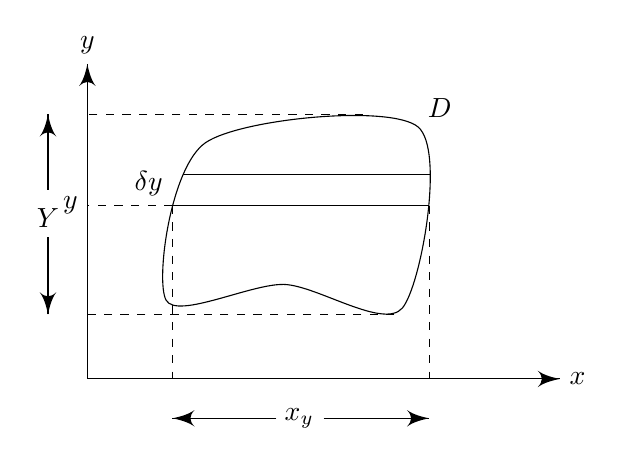
\begin{tikzpicture}
    \draw [->] (0, 0) -- (6, 0) node [right] {$x$};
    \draw [->] (0, 0) -- (0, 4) node [above] {$y$};
    \draw (1.08, 2.2) node [anchor = south east] {$\delta y$} -- (4.34, 2.2);
    \draw (1.22, 2.6) -- (4.36, 2.6);
    \draw [dashed] (1.08, 2.2) -- (1.08, 0);
    \draw [dashed] (4.34, 2.2) -- (4.34, 0);
    \draw [dashed] (1.08, 2.2) -- (0, 2.2) node [left] {$y$};
    \draw [->] (2.4, -0.5) -- (1.08, -0.5);
    \draw [->] (3, -0.5) node [left] {$x_y$} -- (4.34, -0.5);
    \draw plot [smooth cycle] coordinates {(1, 1) (2.5, 1.2) (4, 0.9) (4.2, 3.2) (1.5, 3)};
    \draw [dashed] (3.5, 3.36) -- (0, 3.36);
    \draw [dashed] (3.9, 0.82) -- (0, 0.82);
    \draw [->] (-0.5, 2.4) -- (-0.5, 3.36);
    \draw [->] (-0.5, 1.8) node [above] {$Y$} -- (-0.5, 0.82);
    \node at (4.2, 3.2) [anchor = south west] {$D$};
  \end{tikzpicture}
\end{center}

Sum over all such strips and take $\delta y\to 0$, giving

\begin{prop}
  \[
    \int_D f(x, y)\;\d A = \int_Y\left(\int_{x_y}f(x, y)\;\d x\right) \d y.
  \]
  with $x_y$ ranging over $\{x: (x, y) \in D\}$.
\end{prop}

We could also do it the other way round, integrating over $y$ first, and come up with the result
\[
  \int_D f(x, y)\; \d A = \int_X\left(\int_{y_x}f(x, y)\; \d y\right) \d x.
\]
\begin{thm}[Fubini's theorem]
  If $f$ is a continuous function and $D$ is a compact subset of $\R^2$, then
  \[
    \int\int f\;\d x\;\d y = \int\int f\;\d y\;\d x.
  \]
  This theorem holds in many more cases but those situations have to be checked manually.
\end{thm}
\begin{defi}[Area element]
  The \emph{area element} is $\d A$.
\end{defi}

\begin{prop}
  $\d A = \d x\;\d y$ in Cartesian coordinates.
\end{prop}

\begin{eg}
  We integrate over the triangle bounded by $(0, 0), (2, 0)$ and $(0, 1)$. We want to integrate the function $f(x, y) = x^2y$ over the area. So
  \begin{align*}
    \int _D f(x y)\;\d A &= \int_0^1 \left(\int_0^{2 - 2y}x^2y \;\d x\right)\; \d y\\
    &= \int_0^1 y\left[\frac{x^3}{3}\right]^{2 - 2y}_0 \;\d y\\
    &= \frac{8}{3}\int_0^1 y(1 - y)^3\;\d y\\
    &= \frac{2}{15}
  \end{align*}

  We can integrate it the other way round:
  \begin{align*}
    \int_D x^2 y\;\d A &= \int_0^2 \int_0^{1 - x/2}x^2y \;\d y\;\d x\\
    &= \int_0^2 x^2\left[\frac{1}{2}y^2\right]_0^{1 - x/2}\;\d x\\
    &= \int_0^2 \frac{x^2}{2} \left(1 - \frac{x}{2}\right)^2 \;\d x\\
    &= \frac{2}{15}
  \end{align*}
\end{eg}

Since it doesn't matter whether we integrate $x$ first or $y$ first, if we find it difficult to integrate one way, we can try doing it the other way and see if it is easier.

\note We have a notation with the \emph{range} of a 1-dimensional integral given by a \emph{set}, which may consist of disconnected intervals, eg. $X = [a_1, b_1]\cup [a_2, b_2]$. Then
\[
  \int_X f(x)\; \d x = \int_{a_1}^{b_1} f(x) \;\d x + \int_{a_2}^{b_2}f(x)\;\d x.
\]
This is useful if we want to integrate over a concave area and we have disconnected vertical strips.

\begin{center}
  \begin{tikzpicture}
    \draw [->] (0, 0) -- (6, 0) node [right] {$x$};
    \draw [->] (0, 0) -- (0, 4) node [above] {$y$};
    \draw plot [smooth cycle] coordinates {(1, 1) (4, 0.8) (4.2, 1.1) (3, 2) (4.1, 3) (1.2, 2.7)};
    \draw (3.2, 0.8) -- (3.2, 1.76);
    \draw (3.4, 0.8) -- (3.4, 1.61);
    \draw (3.2, 2.24) -- (3.2, 3.02);
    \draw (3.4, 2.4) -- (3.4, 3.04);
  \end{tikzpicture}
\end{center}

We have a few easy special cases.
\begin{defi}[Separable function]
  A function $f(x, y)$ is separable if it can be written as $f(x, y) = h(y)g(x)$.
\end{defi}

\begin{prop}
  Take separable $f(x, y) = h(y)g(x)$ and $D$ be a rectangle $\{(x, y): a\leq x\leq b, c\leq y \leq d\}$. Then
  \[
    \int_Df(x, y)\;\d x\;\d y = \left(\int_a^b g(x)\;\d x\right)\left(\int_c^d h(y)\;\d y\right)
  \]
\end{prop}

\subsection{Change of variables for an integral in \texorpdfstring{$\R$}{R}}
\begin{prop}
  Suppose we have a change of variables $x(, y)\leftrightarrow (u, v)$ that is smooth and invertible, with regions $D, D'$ in one-to-one correspondence. Then
  \[
    \int_D f(x, y)\;\d x\;\d y = \int_D f(x(u, v), y(u, v))|J|\;\d u\;\d v,
  \]
  where
  \[
    J = \frac{\partial (x, y)}{\partial (u, v)} =
    \begin{vmatrix}
      \dfrac{\partial x}{\partial u} & \dfrac{\partial x}{\partial v}\vspace{5pt}\\
      \dfrac{\partial y}{\partial u} & \dfrac{\partial y}{\partial v}\\
    \end{vmatrix}
  \]
  is the Jacobian. In other words,
  \[
    \;\d x\;\d y = |J|\;\d u\;\d v.
  \]
\end{prop}

\begin{proof}
  Since we are writing $(x(u, v), y(u, v))$, we are actually transforming from $(u, v)$ to $(x, y)$ and not the other way round.

  Suppose we start with an area $\delta A' = \delta u\delta v$ in the $(u, v)$ plane. Then by Taylors, theorem, we have
  \[
    \delta x = x(u + \delta u, v + \delta v) - x(u, v) \approx \frac{\partial x}{\partial u}\delta u + \frac{\partial x}{\partial v}\delta v.
  \]
  We have a similar expression for $\delta y$ and we obtain
  \[
    \begin{pmatrix}
      \delta x\\
      \delta y
    \end{pmatrix}
    \approx
    \begin{pmatrix}
      \frac{\partial x}{\partial u} & \frac{\partial x}{\partial v}\\
      \frac{\partial y}{\partial u} & \frac{\partial y}{\partial v}\\
    \end{pmatrix}
    \begin{pmatrix}
      \delta u\\
      \delta v
    \end{pmatrix}
  \]
  Recall from Vectors and Matrices that the determinant of the matrix is how much it scales up an area. So the area formed by $\delta x$ and $\delta y$ is $|J|$ times the area formed by $\delta u$ and $\delta v$. Hence
  \[
    \d x\;\d y = |J| \;\d u\;\d v.
  \]
\end{proof}

\begin{eg}
  We transform from $(x, y)$ to $(\rho, \varphi)$ with
  \begin{align*}
    x &= \rho\cos \varphi\\
    y &= \rho\sin \varphi
  \end{align*}
  We have previously calculated that $|J| = \rho$. So
  \[
    \d A = \rho \;\d \rho \;\d \varphi.
  \]
  Suppose we want to integrate a function over a quarter area $D$ of radius $R$.
  \begin{center}
    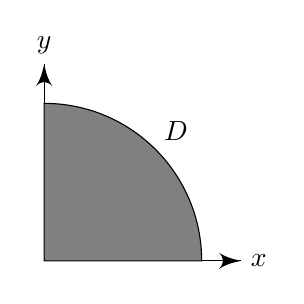
\begin{tikzpicture}
      \draw [->] (0, 0) -- (2.5, 0) node [right] {$x$};
      \draw [->] (0, 0) -- (0, 2.5) node [above] {$y$};
      \draw [fill=gray] (0, 0) -- (2, 0) arc (0:90:2) -- cycle;
      \node at (1.4, 1.4) [anchor=south west] {$D$};
    \end{tikzpicture}
  \end{center}
  Let the function to be integrated be $f = \exp(-(x^2 + y^2)/2) = \exp(-\rho^2/2)$. Then
  \begin{align*}
    \int f\;\d A &= \int f\rho\;\d\rho\;\d\varphi\\
    &=\int_{\rho=0}^R\left(\int_{\varphi=0}^{\pi/2}e^{-\rho^2/2}\rho \;\d \varphi\right)\delta \rho\\
    \intertext{Note that in polar coordinates, we are integrating over a rectangle and the function is separable. So this is equal to}
    &= \left[-e^{-\rho^2/2}\right]^R_0\left[\varphi\right]_0^{\pi/2}\\
    &= \frac{\pi}{2}\left( 1 - e^{-R^2/2}\right).\tag{*}
  \end{align*}
  Note that the integral exists as $R\to \infty$.

  Now we take the case of $x, y\to \infty$ and consider the original integral.
  \begin{align*}
    \int _D f\;\d A &= \int_{x = 0}^{\infty} \int_{y=0}^\infty e^{-(x^2 + y^2)/2}\;\d x\;\d y\\
    &= \left(\int_0^\infty e^{-x^2/2}\;\d x\right)\left(\int_0^\infty e^{-y^2/2}\;\d y\right)\\
    &= \frac{\pi}{2}
  \end{align*}
  where the last line is from (*). So each of the two integrals must be $\sqrt{\pi/2}$, ie.
  \[
    \int_0^\infty e^{-x^2/2}\;\d x = \sqrt{\frac{\pi}{2}}.
  \]

\end{eg}
\subsection{Generalization to \texorpdfstring{$\R^2$}{R2}}
\subsubsection{Definitions}
\begin{defi}[Volume integral]
  Consider a volume $V\in \R^3$ with position vector $\mathbf{r} = (x, y, z)$. We approximate $V$ by $N$ small disjoint subsets of some simple shape (eg. cuboids) labelled by $I$, volume $\delta V_I$, contained within a solid sphere of diameter $\ell$.

  Assume that as $\ell \to 0$ and $N\to \infty$, the union of the small subsets tend to $V$. Then
  \[
    \int_V f(\mathbf{r})\;\d V = \lim_{\ell \to 0} \sum_{I}f(\mathbf{r}_I^*) \delta V_I,
  \]
where $\mathbf{r}_I^*$ is any chosen point in each small subset.
\end{defi}
To evaluate this, we can take $\delta V_I = \delta x \delta y \delta z$, and take $\delta x\to 0$, $\delta y\to 0$ and $\delta z$ in some order. For example, 
\[
  \int_V f(\mathbf{r})\;\d v = \int_D \left(\int_{Z_{xy}}f(x, y, z)\;\d z\right)\;\d x\;\d y.
\]
So we integrate $f(x, y, z)$ over $z$ at each point $(x, y)$, then take the integral of that over the area containing all required $(x, y)$.

Alternatively, we can take the area integral first, and have
\[
  \int_V f(\mathbf{r})\;\d V = \int_z\left(\int_{D_Z} f(x, y, z)\;\d x\;\d y\right)\;\d z.
\]
Again, if we take $f = 1$, then we obtain the volume of $V$.

Often, $f(\mathbf{r})$ is the density of some quantity, and is usually denoted as $\rho$. For example, we might have mass density,charge density, or probability density. $\rho(\mathbf{r})\delta V$ is then the amount of quantity in a small volume $\delta V$ at $\mathbf{r}$. Then $\int_V \rho(\mathbf{r}) \;\d V$ is the total amount of quantity in $V$.

\begin{defi}[Volume element]
  The \emph{volume element} is $\d V$
\end{defi}

\begin{prop}
  $\d V = \d x\; \d y\; \d z$.
\end{prop}

\subsubsection{Change of variables in \texorpdfstring{$\R^3$}{R3}}
We can change variables by some smooth, invertible transformation $(x, y, z)\mapsto (u, v, w)$. Then
\begin{prop}
  \[
    \int_V f\;\d x\;\d y\;\d z = \int_V f|J|\;\d u\;\d v\;\d w,
  \]
  with
  \[
    J = \frac{\partial(x, y, z)}{\partial(u, v, w)} =
    \begin{vmatrix}
      \dfrac{\partial x}{\partial u} & \dfrac{\partial x}{\partial v} & \dfrac{\partial x}{\partial w}\vspace{5pt} \\ 
      \dfrac{\partial y}{\partial u} & \dfrac{\partial y}{\partial v} & \dfrac{\partial y}{\partial w}\vspace{5pt} \\ 
      \dfrac{\partial z}{\partial u} & \dfrac{\partial z}{\partial v} & \dfrac{\partial z}{\partial w}
    \end{vmatrix}
  \]
\end{prop}

In cylindrical coordinates, we have
\begin{align*}
  x &= \rho \cos\varphi\\
  y &= \rho \sin\varphi\\
  z &= z
\end{align*}
So
\begin{prop}
  In cylindrical coordinates,
  \[
    \d V = \rho\;\d \rho\;\d \varphi\;\d z.
  \]
\end{prop}
In spherical coordinates,
\begin{align*}
  x &= r\sin\theta\cos\varphi\\
  y &= r\sin\theta\sin\varphi\\
  z &= r\cos\theta
\end{align*}
So
\begin{prop}
  In spherical coordinates 
  \[
    \d V = r^2\sin\theta \;\d r\;\d \theta\;\d \varphi.
  \]
\end{prop}

\begin{eg}
  Suppose $f(\mathbf{r})$ is spherically symmetric and $V$ is a sphere of radius $a$ centered on the origin. Then
  \begin{align*}
    \int_V f\;\d V &= \int_{r = 0}^a \int_{\theta = 0}^\pi \int_{\varphi = 0}^{2\pi} f(r)r^2 \sin\theta\;\d r\;\d \theta\;\d\varphi\\
    &= \int_0^a \d r\int_0^\pi \d \theta\int_0^{2\pi} \d \varphi \;r^2 f(r) \sin \theta\\
    &= \int_0^a \d r\; r^2 f(r) \Big[-\cos \theta\Big]_0^\pi \Big[\phi\Big]_0^{2\pi}\\
    &= 4\pi\int_0^a f(r)r^2 \;\d r.
  \end{align*}
  where we separated the integral into three parts as in the area integrals.

  Note that in the second line, we rewrote the integrals to write the differentials next to the integral sign. This is simply a different notation that saves us from writing $r = 0$ etc. in the limits of the integrals.

  This is a useful general result. We understand it as the sum of spherical shells of thickness $\delta r$ and volume $4\pi r^2 \delta r$.

  If we take $f = 1$, then we have the familiar result that the volume of a sphere is $\frac{4}{3}\pi a^3$.
\end{eg}

\begin{eg}
  Consider a volume within a sphere of radius $a$ with a cylinder of radius $b$ ($b < a$) removed. The region is defined as
  \begin{align*}
    x^2 + y^2 + z^2 &\leq a^2\\
    x^2 + y^2 &\geq b^2.
  \end{align*} 
  \begin{center}
    \begin{tikzpicture}
      \begin{scope}
        \clip (-.99, 2) rectangle (-3, -2.1) (.99, 2) rectangle (3, -2.1);
        \draw circle [radius=2];
      \end{scope}
      \draw (0, 1.72) circle [x radius=1, y radius = 0.15];
      \draw [dash pattern= on 4pt off 4pt] (1, -1.72) arc (0: 180:1 and 0.15);
      \draw (-1, -1.72) arc (180: 360:1 and 0.15);
      \draw [dash pattern= on 4pt off 4pt] (1, 1.72) -- (1, -1.72);
      \draw [dash pattern= on 4pt off 4pt] (-1, 1.72) -- (-1, -1.72);
      \draw [dash pattern= on 2pt off 2pt] (0, 0) -- (1, 1.72) node [pos = 0.5, anchor = north west] {$a$};
      \draw [dash pattern= on 2pt off 2pt] (0, 0) -- (-1, 0) node [pos = 0.5, above] {$b$};
    \end{tikzpicture}
  \end{center}
  In cylindrical polars, need
  \[
    b \leq \rho \leq a
  \]
  for the $x^2 + y^2 + z^2 \leq a^2$ criterion, we consider how it looks like a point on the surface:
  \begin{center}
    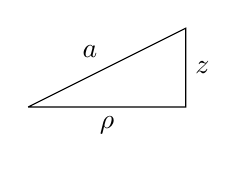
\begin{tikzpicture}
      \draw (0, 0) -- (2, 0) node [pos = 0.5, below] {$\rho$} -- (2, 1) node [pos = 0.5, right] {$z$} -- (0, 0) node [pos = 0.5, anchor = south east] {$a$};
    \end{tikzpicture}
  \end{center}
  and obtain
  \[
    -\sqrt{a^2 - \rho^2} \leq z \leq \sqrt{a^2 - \rho^2}.
  \]
  So the volume is
  \begin{align*}
    \int_V \;\d V &= \int_b^a\d \rho\int_0^{2\pi}\d \varphi \int_{-\sqrt{a^2 - \rho^2}}^{\sqrt{a^2 - \rho^2}}\d z\; \rho\\
    &= 2\pi\int_b^a 2\rho\sqrt{a^2 - \rho^2}\;\d \rho\\
    &= 2\pi \left[\frac{2}{3}(a^2 - \rho^2)^{3/2}\right]^a_b\\
    &= \frac{4}{3}\pi (a^2 - b^2)^{3/2}.
  \end{align*}
\end{eg}
\begin{eg}
  Suppose the density of electric charge $\rho(\mathbf{r}) = \mathbf{r}_0 \frac{z}{a}$ in a hemisphere $H$ of radius $a$, with $z \geq 0$. What is the total charge of $H$?

  We use spherical polars. So
  \[
    V \leq a,\quad 0 \leq \phi \leq 2\pi,\quad 0 \leq \theta \leq \frac{\pi}{2}.
  \]
  We have
  \[
    \rho(\mathbf{r}) = \frac{\rho_0}{a}r\cos \theta.
  \]
  The total charge $Q$ in $H$ is
\begin{align*}
  \int_H \rho \;\d V &= \int_0^a\d r\int_0^{\pi/2}\d \theta\int_0^{2\pi}\d\varphi\; \frac{\rho_0}{a}r\cos\theta r^2\sin\theta\\
  &= \frac{\rho_0}{a}\int_0^a r^3 \;\d r = \int_0^{\pi/2}\sin\theta \cos\theta\;\d \theta \int_0^{2\pi}\;\d \varphi\\
  &= \frac{\rho_0}{a}[r^4/4]^a_0\left[\frac{1}{2}\sin^2\theta\right]^{\pi/2}_0 [\varphi]^{2\pi}_0\\
  &= \frac{\rho_0 \pi a^3}{4}.
\end{align*}
\end{eg}
\subsection{Further generalizations}
\subsubsection{Integration in \texorpdfstring{$R^n$}{Rn}}
$\int_D f(x_1, x_2, \cdots x_n)\;\d x_1 \;\d x_2\cdots\;\d x_n$ is simply the integration over an $n$-dimensional volume. The change of variable formula is
\begin{prop}
  \[
    \int_D f(x_1, x_2, \cdots x_n)\;\d x_1 \;\d x_2\cdots\;\d x_n = \int_{D'} f(\{x_i(\mathbf{u})\}) |J| \;\d u_1\;\d u_2\cdots\;\d u_n.
  \]
\end{prop}

\subsubsection{Change of variables for \texorpdfstring{$n = 1$}{n = 1}}
In the $n = 1$ case, the Jacobian is $\frac{\d x}{\d u}$. However, we use the following formula for change of variables:
\[
  \int_D f(x) \;\d x = \int_{D'} f(x(u))\left|\frac{\d x}{\d u}\right| \;\d u.
\]
This modulus is correct because of our natural convention about integrating over $D$ and $D'$, i.e. we use the numerically smaller bound as the lower bound.

Supposed the original bounds are $a$ and $b$, and are mapped to $\alpha, \beta$. If $a < b$ and $\alpha < \beta$, then $\frac{\d x}{\d u}$ is positive, and we have, as expected
\[
  \int_a^b f(x)\;\d x = \int_\alpha^\beta f(u)\frac{\d x}{\d u}\;\d u.
\]
If $\alpha > \beta$, then $\frac{\d x}{\d u}$ is negative. So
\[
  \int_a^b f(x)\;\d x = \int_\alpha^\beta f(u)\frac{\d x}{\d u}\;\d u = \int_\beta^\alpha f(u)-\frac{\d x}{\d u}\;\d u.
\]
By taking the absolute value of $\frac{\d x}{\d u}$, we ensure that we always have the numerically smaller bound as the lower bound.

This is not easily generalized to higher dimensions, so we don't employ the same trick in other cases.

\subsubsection{Vector valued integrals}
We can define $\int_V \mathbf{F}(\mathbf{r})\;\d V$ in a similar way to $\int_V f(\mathbf{r})\;\d V$as the limit of a sum over small contributions of volume. In practice, we integrate them componentwise. If
\[
  \mathbf{F}(\mathbf{r}) = F_{i(\mathbf{r})}\mathbf{e}_i,
\]
then
\[
  \int_V \mathbf{F}(\mathbf{r})\;\d V = \int_V (F_i(\mathbf{r})\;\d V)\mathbf{e}_i.
\]
For example, if a mass has density $\rho (\mathbf{r})$, then its mass is
\[
  M = \int_V \rho(\mathbf{r})\;\d V
\]
and its center of mass is
\[
  \mathbf{R} = \frac{1}{M}\int_V \mathbf{r}\rho (\mathbf{r})\;\d V.
\]
\begin{eg}
  Consider a solid hemisphere $H$ with $r \leq a$, $z \geq 0$ with uniform density $\rho$. The mass is
  \[
    M = \int_H \rho \;\d V = \frac{2}{3}\pi a^3\rho.
  \]
  Now suppose that $\mathbf{R} = (X, Y, Z)$. By symmetry, we expect $X = Y = 0$. We can find this formally by
\begin{align*}
  X &= \frac{1}{M}\int_H x\rho \;\d V\\
  &= \frac{\rho}{M}\int_0^a \int_0^{\pi/2}\int_0^{2\pi}xr^2 \sin \theta\;\d \varphi\;\d \theta\;\d r\\
  &= \frac{\rho}{M}\int_0^{a}r^3\;\d r\times \int_0^{\pi/2}\sin^2\theta\;\d \theta\times \int_0^{2\pi}\cos\varphi\;\d \varphi\\
  &= 0
\end{align*}
as expected. Note that it evaluates to 0 because the integral of $\cos$ from $0$ to $2\pi$ is 0. Similarly, we obtain $Y = 0$.

Finally, we find $Z$.
\begin{align*}
  Z &= \frac{\rho}{M}\int_0^a r^3\;\d r \int_0^{\pi/2}\sin\theta\cos\theta\;\d \theta \int_0^{2\pi}\;\d \varphi\\
  &= \frac{r}{M}\left[\frac{a^4}{4}\right]\left[\frac{1}{2}\sin^2\theta\right]_0^{\pi/2}2\pi\\
  &= \frac{3a}{8}. 
\end{align*}
So $\mathbf{R} = (0, 0, 3a/8)$.
\end{eg}

\section{Surfaces and surface integrals}
\subsection{Surfaces and Normal}
Let $f$ be a smooth function on $\R^3$ and a constant $c$. Then $f(\mathbf{r}) = c$. defines a smooth surface. Consider any curve $\mathbf{r}(u)$ in $S$. Then by the chain rule, if we differentiate $f(\mathbf{r}) = c$ with respect to $u$, we obtain
\[
  \frac{\d }{\d u}[f(\mathbf{r}(u))] = \nabla f\cdot \frac{\d \mathbf{r}}{\d u} = 0.
\]
This means that $\nabla f$ is always perpendicular to $\frac{\d \mathbf{r}}{\d u}$. We know that $\frac{\d \mathbf{r}}{\d u}$ is the tangent to the curve. So $\nabla f$ is perpendicular to the tangent. Since this is true for any curve $\mathbf{r}(u)$, $\nabla f$ is perpendicular to any tangent of the surface. Therefore
\begin{prop}
  $\nabla f$ is the normal to the surface $f(\mathbf{r}) = c$.
\end{prop}

\begin{eg}\leavevmode
  \begin{enumerate}
    \item Take the sphere $f(\mathbf{r}) = x^2 + y^2 + z^2 = c$ for $c > 0$. Then $\nabla f = 2(x, y, z) = 2\mathbf{r}$, which is clearly normal to the sphere.
    \item Take $f(\mathbf{r}) = x^2 + y^2 - z^2 = c$, which is a hyperboloid. Then $\nabla f = 2(x, y, -z)$. If $c = 0$, then we have a double cone, with a singular apex $\mathbf{0}$, where $\nabla f = 0$.
  \end{enumerate}
\end{eg}

\begin{defi}[Boundary]
  A surface $S$ can be defined to have a \emph{boundary} $\partial S$ consisting of a piecewise smooth curve. If we define $S$ as in the above examples but with the additional restriction $z \geq 0$, then $\partial S$ is the circle $x^2 + y^2 = c$, $z = 0$.

  A surface is \emph{bounded} if it can be contained in a solid sphere, \emph{unbounded} otherwise. A bounded surface with no boundary is called \emph{closed}. (e.g. sphere)
\end{defi}

\begin{defi}[Orientable surface]
  At each point, there is a unit normal $\mathbf{n}$ that's unique up to a sign. The surface is \emph{orientable} if there is a consistent choice of $\mathbf{n}$ which varies smoothly.

  For an orientable surface, the unit normal is determined everywhere by a choice of sign. This sign is called the \emph{orientation} of the surface.
\end{defi}
An example of a non-orientable surface is the Mobius strip.

For simple cases, we can describe the orientation as ``inward'' and ``outward''.

\subsection{Parametrized surfaces and area}
A surface $S$ can also be parametrised by $\mathbf{r}(u, v)$ with parameters $u, v$. $S$ is swept out as $u$ and $v$ vary in some region $D$. By the chain rule, 
\[
  \delta r = \frac{\partial \mathbf{r}}{\partial u}\delta u + \frac{\partial \mathbf{r}}{\delta v} + o(\delta u, \delta v).
\]
$\frac{\partial \mathbf{r}}{\delta u}$ and $\frac{\partial \mathbf{r}}{\partial v}$ are tangent vectors to curves on $S$ with $v, u$ constant, respectively.

\begin{defi}[Regular parametrization]
  A parametrization is \emph{regular} if for all $u, v$,
  \[
    \frac{\partial \mathbf{r}}{\partial u}\times \frac{\partial \mathbf{r}}{\partial v} \not = 0,
  \]
  ie. there are always two independent tangent directions.
\end{defi}

The small changes $\delta u, \delta v$ make a small parallelogram on $S$, up to $o$-terms, it has a vector area of 
\[
  \delta \mathbf{S} = \frac{\partial \mathbf{r}}{\delta u}\times \frac{\partial \mathbf{r}}{\partial v} = \delta S \mathbf{n}.
\]
The order of $u, v$ gives the choice of unit normal. By summing and taking limits, the area of $S$ is
\[
  \int_S \d S  = \int_D \left|\frac{\partial \mathbf{r}}{\partial u}\times \frac{\partial \mathbf{r}}{\partial v}\right| \d u\;\d v
\]
\begin{prop}
  \[
    \d S = \left|\frac{\partial \mathbf{r}}{\partial u}\times \frac{\partial \mathbf{r}}{\partial v}\right|\;\d u\;\d v
  \]
  is the \emph{scalar area element}.
\end{prop}

\begin{eg}
  Let $S$ be part of a sphere of radius $a$. Then %insert diagram, hemisphere up to $\theta = \alpha$..
  \[
    \mathbf{r}(\theta, \varphi) = (a\cos\varphi\sin \theta, a\sin \theta\sin \varphi, a\cos \theta) = a\mathbf{e}_r.
  \]
  Then
  \[
    \frac{\partial \mathbf{r}}{\partial \theta} = a\mathbf{e}_\theta.
  \]
  and similarly for $\varphi$. Then, after some tedious algebra,
  \[
    \left|\frac{\partial \mathbf{r}}{\partial u}\times \frac{\partial \mathbf{r}}{\partial v}\right| = a^2\sin \theta \mathbf{e}_r.
  \]
  So
  \[
    \d S = a^2\sin \theta\;\d \theta\;\d \varphi.
  \]
  Our bounds is $0 \leq \theta < \alpha$, $0 \leq \varphi \leq 2\pi$.

  Then the area is
  \[
    \int_0^{2\pi}\int_0^{\alpha} a^2\sin \theta\;\d \phi \;\d \theta = 2\pi a^2(1 - \cos\alpha).
  \]
\end{eg}
\subsection{Surface integral of vector fields}
Let $S$ be a smooth surface: $\mathbf{r}(u, v)$ with $S$ corresponding to a region in $(u, v)$ parameter space.
\begin{defi}[Surface integral]
  The \emph{surface integral} or $\emph{flux}$ of a vector field $\mathbf{F}(\mathbf{r})$ over $S$ is defined by
  \[
    \int_S \mathbf{F}(\mathbf{r})\cdot \d \mathbf{S} = \int_S \mathbf{F}(\mathbf{r})\cdot \mathbf{n}\;\d S = \int_D \mathbf{F}(\mathbf{r}(u, v))\cdot \left(\frac{\partial \mathbf{r}}{\partial u}\times \frac{\partial \mathbf{r}}{\partial v}\right)\;\d u\;\d v.
  \]
  Intuitively, this is the total amount of $\mathbf{F}$ passing through $S$. For example, if $\mathbf{F}$ is the electric field, the flux is the amount of electric field passing through a surface.
\end{defi}

For a given orientation, the integral $\int \mathbf{F}\cdot \mathbf{S}$ is independent of the parametrization. Changing orientation is equivalent to changing the sign of $\mathbf{n}$, which is in turn equivalent to changing the order of $u$ and $v$ in the definition of $S$, which is also equivalent to changing the sign of the flux integral.

\begin{eg}
  Consider a sphere of radius $a$, $\mathbf{r}(\theta, \varphi)$. Then
  \[
    \frac{\partial \mathbf{r}}{\partial \theta} = a\mathbf{r}_\theta,\quad \frac{\partial \mathbf{r}}{\partial \varphi} = a\sin \theta \mathbf{e}_\varphi.
  \]
  The vector area element is
  \[
    \d \mathbf{S} = a^2\sin \theta \mathbf{e}_r \;\d \theta\; \d\varphi.
  \]
  with $\mathbf{n} = \mathbf{e}_r = \mathbf{r}/a$, which is an outward normal.

  Suppose we ant to calculate the fluid flux through the surface. The \emph{velocity field} $\mathbf{u}(\mathbf{r})$ of a fluid gives the motion of a small volume of fluid $\mathbf{r}$. Assume that $\mathbf{u}$ depends smoothly on $\mathbf{r}$ (and $t$). For any small area $\delta S$, on a surface $S$, the volume of fluid crossing it in time $\delta t$ is $\mathbf{u}\cdot \delta S\; \delta t$.
\begin{center}
  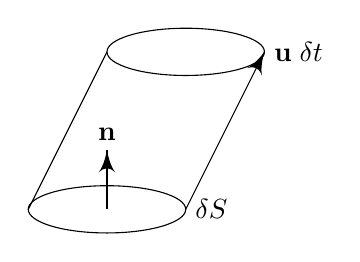
\begin{tikzpicture}
    \draw circle [x radius = 1, y radius = 0.3];
    \node at (1, 0) [right] {$\delta S$};
    \draw (1, 2) circle [x radius = 1, y radius = 0.3];
    \draw (-1, 0) -- (0, 2);
    \draw [->] (1, 0) -- (2, 2) node [right] {$\mathbf{u}\;\delta t$};
    \draw [->] (0, 0) -- (0, .75) node [above] {$\mathbf{n}$};
  \end{tikzpicture}
\end{center}
So the flux of $\mathbf{u}$ over at time $\delta t$ is
\[
  \delta t\int_S \mathbf{u}\cdot \d \mathbf{S}.
\]
So $\int_S \mathbf{u}\cdot \d \mathbf{S}$ is the \emph{rate} of volume crossing $S$.

For example, let $\mathbf{u} = (-x, 0, z)$ and $S$ be the section of a sphere of radius $a$ with $0 \leq \varphi \leq$ and $0 \leq \theta \leq \alpha$. Then
\[
  \d \mathbf{S} = a^2 \sin \theta \mathbf{n}\;\d \varphi \;\d \theta,
\]
with 
\[
  \mathbf{n} = \frac{\mathbf{r}}{a} = \frac{1}{a}(x, y, z).
\]
So
\[
  \mathbf{n}\cdot \mathbf{u} = \frac{1}{a}(-x^2 + z^2) = a(-\sin^2\theta\cos^2\varphi + \cos^2 \theta).
\]
Therefore
\begin{align*}
  \int_S \mathbf{u}\cdot \d \mathbf{S} &= \int_0^\alpha \int_0^{2\pi} a^3 \sin \theta[(\cos^2\theta - 1) \cos^2 \varphi + \cos^2 \theta]\;\d \varphi\;\d \theta\\
  &= \int_0^\alpha a^3\sin \theta[\pi(cos^2\theta - 1) + 2\pi \cos^2\theta]\; \d \theta\\
  &=\int_0^\alpha a^3\pi(3\cos^3 \theta - 1)\sin \theta\;\d \theta\\
  &= \pi a^3[cos\theta - \cos^3 \theta]_0^\alpha\\
  &= \pi a^3 \cos \alpha\sin^2 \alpha.
\end{align*}
\end{eg}

Any change in parametrization is done explicitly. Let $\mathbf{r}(u, v)$ and $\mathbf{r}(\tilde{u}, \tilde{v})$ be two regular parametrizations for the surface. By the chain rule,
\begin{align*}
  \frac{\partial \mathbf{r}}{\partial u} &= \frac{\partial \mathbf{r}}{\partial \tilde{u}}\frac{\partial\tilde{u}}{\partial u} + \frac{\partial \mathbf{r}}{\partial \tilde{v}}\frac{\partial\tilde{v}}{\partial u}\\
  \frac{\partial \mathbf{r}}{\partial v} &= \frac{\partial \mathbf{r}}{\partial \tilde{u}}\frac{\partial\tilde{u}}{\partial v} + \frac{\partial \mathbf{r}}{\partial \tilde{v}}\frac{\partial\tilde{v}}{\partial v}
\end{align*}
So
\[
  \frac{\partial \mathbf{r}}{\partial u}\times\frac{\partial\mathbf{r}}{\partial v} = \frac{\partial (\tilde{u}, \tilde{v})}{\partial (u, v)} \frac{\partial \mathbf{r}}{\partial \tilde {u}}\times\frac{\partial\mathbf{r}}{\partial \tilde{v}}
\]
Then
\begin{prop}
  The \emph{scalar area element} is
  \[
    \d S = \left|\frac{\partial \mathbf{r}}{\partial u}\times\frac{\partial\mathbf{r}}{\partial v}\right|\;\d u\;\d v = \left|\frac{\partial \mathbf{r}}{\partial \tilde {u}}\times\frac{\partial\mathbf{r}}{\partial \tilde{v}}\right| \;\d \tilde{u}\;\d \tilde{v}.
  \]
\end{prop}
Similarly, we have
\begin{prop}
  The \emph{vector area element} is
  \[
    \d \mathbf{S} = \frac{\partial \mathbf{r}}{\partial u}\times\frac{\partial\mathbf{r}}{\partial v}\;\d u\;\d v = \frac{\partial \mathbf{r}}{\partial \tilde {u}}\times\frac{\partial\mathbf{r}}{\partial \tilde{v}} \;\d \tilde{u}\;\d \tilde{v}.
  \]
  provided $(u, v)$ and $(\tilde{u}, \tilde{v})$ have the same orientation.
\end{prop}
\subsection{Comparing line, surface, and volume integrals}
We have analogous definitions for integrals of scalar functions $f$ or vector functions $\mathbf{F}$ along a curve or surface.

\begin{tabular}[]{p{0.4\textwidth}p{0.4\textwidth}}
  \toprule
  Scalar function & Vector function\\
  \midrule
  $\displaystyle \int_C f\;\d s$ & $\displaystyle \int_C \mathbf{F}\cdot \d \mathbf{r} = \int_C \mathbf{F}\cdot \mathbf{r}\;\d s$\vspace{5pt}\\
  $\displaystyle \int_S f\;\d S$ & $\displaystyle \int_S \mathbf{S}\cdot \d \mathbf{S} = \int_S \mathbf{F}\cdot \mathbf{n} \;\d S$\\
  \midrule
  Independent of orientation. $f = 1$ gives length or area & Depends on orientation from the definition of the integral \emph{or} the choice of unit tangent or normal.\\
  \bottomrule
\end{tabular}

By convention, the limits on $u, v$ integrals are in the natural order, i.e. $\alpha < \beta$ with $\alpha < \beta$ except for the $\d \mathbf{r}$ integral, where we do not change the order. 

\subsection{Change of variables in \texorpdfstring{$\R^2$ and $\R^3$}{R2 and R3} revisited}
In this section, we derive our change of variable formulae in a slightly different way.

\subsubsection{Change of variable formula in \texorpdfstring{$\R^2$}{R2}}
We first derive the 2D change of variable formula from the 3D surface integral formula.

Consider a subset $S$ of the plane $\R^2$ parametrized by $\mathbf{r}(x(u, v), y(u, v))$. We can embed it to $\R^3$ as $\mathbf{r}(x(u, v), y(u, v), 0)$. Then
\[
  \frac{\partial \mathbf{r}}{\partial u}\times \frac{\partial\mathbf{r}}{\partial v} = (0, 0, J),
\]
with $J$ being the Jacobian.
Therefore 
\[
  \int_S f(\mathbf{r})\;\d S = \int_D f(\mathbf{r}(u, v)) \frac{\partial \mathbf{r}}{\partial u}\times \frac{\partial \mathbf{r}}{\partial u} = \int_D f(\mathbf{r}(u, v))|J|\;\d u\;\d v
\]
and we recover the formula for changing variables in $\R^2$.

\subsubsection{Change of variable formula in \texorpdfstring{$R^3$}{R3}}
In $\R^3$, suppose we have a volume parametrised by $\mathbf{r}(u, v, w)$. Then
\[
  \d \mathbf{r} = \frac{\partial \mathbf{r}}{\partial u}\delta u + \frac{\partial \mathbf{r}}{\partial v}\delta v + \frac{\partial \mathbf{r}}{\partial w}\delta w + o(\delta u, \delta v, \delta w).
\]
Then the cuboid $\delta u, \delta v, \delta w$ in $u, v, w$ space is mapped to a parallelopiped of volume
\[
  \delta V = \left|\frac{\partial \mathbf{r}}{\partial u}\delta u\cdot \left( \frac{\partial \mathbf{r}}{\partial v}\delta v \times \frac{\partial \mathbf{r}}{\partial w}\delta w\right)\right| = |J|\;\delta u\; \delta v\;\delta w.
\]
So $\d V = |J|\; \d u\; \d v\; \d w$.

\section{Geometry of curves and surfaces}
Let $\mathbf{r}(s)$ be a curve parametrized by arclength $s$. Since $\mathbf{t}(s) = \frac{\d \mathbf{r}}{\d s}$ is a unit vector, $\mathbf{t}\cdot \mathbf{t} = 1$. Differentiating yields $\mathbf{t}\cdot \mathbf{t}' = 0$. So $\mathbf{t}'$ is a normal to thee curve if $\mathbf{t}' \not= 0$.

We define the following:
\begin{defi}[Principal normal and curvature]
Let $\mathbf{t}' = \kappa \mathbf{n}$, where the unit vector $\mathbf{n}(s)$ is called the \emph{principal normal}. $\kappa(s)$ is called the \emph{curvature}. We make $\kappa > 0$ by choosing an appropriate direction for $\mathbf{n}$.
\end{defi}

We take a curve that can Taylor expanded around $s = 0$. Then
\[
  \mathbf{r}(s) = \mathbf{r}(0) + s\mathbf{r}'(0) + \frac{1}{2}s^2 \mathbf{r}''(0) + O(s^3).
\]
We know that $\mathbf{r}' = \mathbf{t}$ and $\mathbf{r}'' = \mathbf{t}'$. So we have
\[
  \mathbf{r}(s) = \mathbf{r}(0) + s\mathbf{t}(0) + \frac{1}{2}\kappa(0) s^2 \mathbf{n} + O(s^3).
\]
How can we interpret $\kappa$ as the curvature? Suppose we want to approximate the curve near $\mathbf{r}(0)$ by a circle. We would expect a more ``curved'' curve would be approximated by a circle of smaller radius. So $\kappa$ should be inversely proportional to the radius of the circle. In fact, we will show that $\kappa = 1/a$, where $a$ is the radius of the best-fit circle.

Consider the vector equation for a circle passing through $\mathbf{r}(0)$ with radius $a$ in the plane defined by $\mathbf{t}$ and $\mathbf{n}$.

\begin{center}
  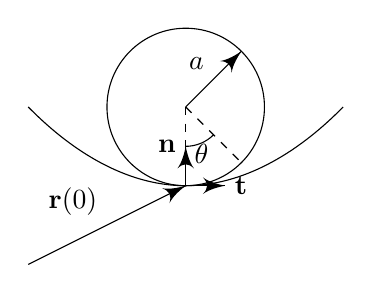
\begin{tikzpicture}
    \draw circle [radius = 1];
    \draw [->] (0, 0) -- (0.707, 0.707) node [anchor = south east, pos = 0.5] {$a$};
    \draw [->] (-2, -2) -- (0, -1) node [anchor = south east, pos = 0.5] {$\mathbf{r}(0)$};
    \draw [->] (0, -1) -- (0.5, -1) node [right] {$\mathbf{t}$};
    \draw [->] (0, -1) -- (0, -0.5) node [left] {$\mathbf{n}$};
    \draw [dashed] (0, 0) -- (0, -1);
    \draw [dashed] (0, 0) -- (0.707, -0.707);
    \draw (0, -0.5) arc (270:315:0.5);
    \node at (0.2, -0.6) {$\theta$};
    \draw (-2, 0) parabola bend (0, -1) (2, 0);
  \end{tikzpicture}
\end{center}
Then the equation of the circle is
\[
  \mathbf{r} = \mathbf{r}(0) + a(1 - \cos \theta) \mathbf{n} + a\sin \theta \mathbf{t}.
\]
We can expand this to obtain
\[
  \mathbf{r} = \mathbf{r}(0) + a\theta t + \frac{1}{2}\theta^2 a\mathbf{n} + o(\theta^3).
\]
Since the arclength $s = a\theta$, we obtain
\[
  \mathbf{r} = \mathbf{r}(0) + s\mathbf{t} + \frac{1}{2}\frac{1}{a}s^2\mathbf{n} + O(s^3).
\]
As promised, $\kappa = 1/a$, for $a$ being the radius of the circle of best fit.

\begin{defi}[Radius of curvature]
  The \emph{radius of curvature} of a curve at a point $\mathbf{r}(s)$ is $1/\kappa(s)$.
\end{defi}

In practice, for $\mathbf{r}(u)$ given in terms of parameter $u$, we can calculate $\mathbf{t}, s, \mathbf{n}, \kappa$ by taking $\frac{\d }{\d u}$ and the use the chain rule.

Since we are in 3D, given $\mathbf{t}(s)$ and $\mathbf{n}(s)$, there is another normal to the curve. We can add a third normal to generate an orthonormal basis.
\begin{defi}[Binormal]
  The \emph{binormal} of a curve is $\mathbf{b} = \mathbf{t}\times \mathbf{n}$.
\end{defi}

The geometry of the curve is encoded in how this basis ($\mathbf{t}, \mathbf{n}, \mathbf{b}$) changes along it. This can be specified by two scalar functions of arc length - the curvature $\kappa(s)$ and the \emph{torsion} $\tau(s)$ (which determines what the curve looks like to third order in its Taylor expansions and how the curve lifts out of the $\mathbf{t}, \mathbf{r}$ plane).

\subsection{Surfaces and intrinsic geometry*}
We can study the geometry of surfaces through curves which lie on them. At a given point $P$ at a surface $S$ with normal $\mathbf{n}$, consider a plane containing $\mathbf{n}$. The intersection of the plane with the surface yields a curve on the surface through $P$. This curve has a curvature $\kappa$ at $P$.

If we choose different planes containing $\mathbf{n}$, we end up with different curves of different curvature. Then we define the following:
\begin{defi}[Principal curvature]
  The \emph{principal curvatures} of a surface at $P$ are the minimum and maximum possible curvature of a curve through $P$, denoted $\kappa_{\min}$ and $\kappa_{\max}$ respectively.
\end{defi}

\begin{defi}[Gaussian curvature]
  The \emph{Gaussian curvature} of a surface at a point $P$ is $K = \kappa_{\min}\kappa_{\max}$.
\end{defi}

\begin{thm}[Theorema Egregium]
  $K$ is \emph{intrinsic} to the surface $S$. It can be expressed in terms of lengths, angles etc. which are measured entirely on the surface. So $K$ can be defined on an arbitrary surface without embedding it on a higher dimension surface.
\end{thm}
The is the start of \emph{intrinsic geometry}: if we embed a surface in Euclidean space, we can determine lengths, angles etc on it. But We don't have to do so - we can ``live in '' the surface and do geometry in it without an embedding.

For example, we can consider a geodesic triangle $D$ on a surface $S$. It consists of three geodesics: shortest curves between two points.

Let $\theta_i$ be the interior angles of the triangle (defined by using scalar products of tangent vectors). Then
\begin{thm}[Guass-Bonet theorem]
  \[
    \theta_1 +\theta_2 + \theta_3 = \pi + \int_D K\; \d A,
  \]
  integrating over the area of the triangle.
\end{thm}

\section{Div, Grad, Curl and \texorpdfstring{$\nabla$}{nabla}}
We regard the gradient $\nabla f$ as obtained from the scalar field $f$ by applying
\[
  \nabla = \mathbf{e}_i \frac{\partial}{\partial x_i}
\]
for cartesian coordinates $x_i$ and orthonormal basis $\mathbf{e}_i$. We can alternatively write this as
\[
  \nabla = \left(\frac{\partial}{\partial x}, \frac{\partial }{\partial y}, \frac{\partial}{\partial z}\right).
\]
where $\mathbf{e}_i$ are orthonormal and right-handed, ie. $\mathbf{e}_i\times \mathbf{e}_j = \varepsilon_{ijk} \mathbf{e}_k$ (it is left handed if $\mathbf{e}_i\times \mathbf{e}_j = -\varepsilon_{ijk} \mathbf{e}_k$).

$\nabla$ (\emph{nabla} or \emph{del}) is both an operator and a vector. We can apply it to a vector field $\mathbf{f}(\mathbf{r}) = \mathbf{F}_i(\mathbf{r})\mathbf{e}_i$ using the scalar or vector product.

\begin{defi}[Divergence]
  The \emph{divergence} or \emph{div} of $\mathbf{F}$ is
  \[
    \nabla\cdot \mathbf{F} = \frac{\partial F_i}{\partial x_i} = \frac{\partial F_1}{\partial x_1} + \frac{\partial F_2}{\partial x_2} + \frac{\partial F_3}{\partial x_3}.
  \]
\end{defi}

\begin{defi}[Curl]
  The \emph{curl} of $\mathbf{F}$ is
  \[
    \nabla\times \mathbf{F} = \varepsilon_{ijk}\frac{\partial F_i}{\partial x_i}\mathbf{e}_i = \begin{vmatrix}
      \mathbf{e}_1 & \mathbf{e}_2 & \mathbf{3}_3\\
      \frac{\partial}{\partial x} & \frac{\partial}{\partial y} & \frac{\partial}{\partial z}\\
      F_x & F_y & F_z
    \end{vmatrix}
  \]
\end{defi}

\begin{eg}
  Let $\mathbf{F} = (xe^z, y^2\sin x, xyz)$. Then
  \[
    \nabla \mathbf{F} = \frac{\partial }{\partial x}(xe^z) + \frac{\partial}{\partial y}y^2 \sin x + \frac{\partial}{\partial z}xyz = e^z + 2y\sin x + xy.
  \]
  and
  \begin{align*}
    \nabla \times F &= \hat{\mathbf{i}} \left[\frac{\partial}{\partial y}(xyz) - \frac{\partial}{\partial z}y^2\sin x)\right]\\
    &+ \hat{\mathbf{j}} \left[\frac{\partial}{\partial z}(xe^z) + \frac{\partial}{\partial x}(xyz)\right]\\
    &+ \hat{\mathbf{k}}\left[\frac{\partial}{\partial x}(y^2\sin x) - \frac{\partial}{\partial y} (xe^z)\right]\\
    &= (xz, xe^z - yz, y^2\cos x).
  \end{align*}
\end{eg}
Note that $\nabla$ is an operator, so ordering is important. For example,
\[
  F\cdot \nabla = F_i\frac{\partial }{\partial x_i}
\]
is a scalar differential operator, and
\[
  F\times \nabla = \mathbf{e}_k\varepsilon_{ijk}F_i\frac{\partial}{\partial x_j}
\]
is a vector differential operator.

\begin{prop}
  Let $f, g$ be scalar functions, $\mathbf{F}, \mathbf{G}$ be vector functions, and $\mu, \lambda$ be constants. Then
  \begin{align*}
    \nabla(\lambda f + \mu g) &= \lambda\nabla f + \mu\nabla g\\
    \nabla\cdot (\lambda \mathbf{F} + \mu \mathbf{G}) &= \lambda\nabla \cdot \mathbf{F} + \mu\nabla\cdot \mathbf{G}\\
    \nabla\times (\lambda \mathbf{F} + \mu \mathbf{G}) &= \lambda\nabla\times \mathbf{F} + \mu\nabla\times \mathbf{G}.
  \end{align*}
\end{prop}

Note that Grad and Div can be analogously defined in any dimension $n$, but curl is specific to $n = 3$ because it uses the vector product.

\begin{eg}
  Consider $r^\alpha$ with $r = |\mathbf{r}|$. We know that $\mathbf{r}= x_i\mathbf{e}_i$. So $r^2 = x_ix_i$. Therefore
  \[
    2r\frac{\partial r}{\partial x_j} = 2x_j,
  \]
  or
  \[
    \frac{\partial r}{\partial x_i} = \frac{x_i}{r}.
  \]
  So
  \[
    \nabla r^\alpha = \mathbf{e}_i \frac{\partial}{\partial x_i}(r^\alpha) = \mathbf{e}_i\alpha r^{\alpha - 1}\frac{\partial r}{\partial x_i} = \alpha r^{\alpha - 2}\mathbf{r}.
  \]
  Also,
  \[
    \nabla\cdot \mathbf{r} = \frac{\partial x_i}{\partial x_i} = 3.
  \]
  and
  \[
    \nabla \times \mathbf{r} = \mathbf{e}_k \varepsilon_{ijk}\frac{\partial x_j}{x_i} = 0.
  \]
\end{eg}

\begin{prop}
  We have the following Leibnitz properties:
  \begin{align*}
    \nabla(fg) &= (\nabla f)g + f(\nabla g)\\\
    \nabla\cdot (f\mathbf{F}) &= (\nabla f)\cdot \mathbf{F} + f(\nabla\cdot \mathbf{F})\\
    \nabla\times (f\mathbf{F}) &= (\nabla f)\times \mathbf{F} + f(\nabla\times \mathbf{F})\\
    \nabla(\mathbf{F}\cdot \mathbf{G}) &= \mathbf{F}\times (\nabla \times G) + \mathbf{G}\times (\nabla \times \mathbf{F}) + (\mathbf{F}\cdot \nabla)\mathbf{G} + (\mathbf{G}\cdot \nabla) \mathbf{F}\\
    \nabla \times (\mathbf{F}\times G) &= \mathbf{F}(\nabla\cdot \mathbf{G}) - \mathbf{G}(\nabla\cdot \mathbf{F}) + (\mathbf{G}\cdot \nabla)\mathbf{F} - (\mathbf{F}\cdot \nabla)\mathbf{G}\\
    \nabla\cdot (\mathbf{F}\times \mathbf{G}) &= (\nabla\times \mathbf{F})\cdot \mathbf{G} - \mathbf{F}\cdot (\nabla\times \mathbf{G})
  \end{align*}
\end{prop}
which can be proven by brute-forcing with suffix notation and summation convention.

\begin{eg}
  \begin{align*}
    \nabla\cdot (r^\alpha \mathbf{r}) &= (\nabla r^\alpha)\mathbf{r} + r^\alpha \nabla\cdot \mathbf{r}\\
    &= (\alpha r^{\alpha - 2}\mathbf{r})\cdot \mathbf{r} + r^\alpha (3)\\
    &= (\alpha + 3)r^\alpha\\
    \nabla\times (r^\alpha \mathbf{r}) &= (\nabla(r^\alpha))\times \mathbf{r} + r^\alpha(\nabla\times \mathbf{r})\\
    &= \alpha r^{\alpha - 2} \mathbf{r}\times \mathbf{r}\\
    &= 0
  \end{align*}
\end{eg}
\subsection{Second-order derivatives}
We have
\begin{prop}
  \begin{align*}
    \nabla\times (\nabla f) &= 0\\
    \nabla\cdot (\nabla\times \mathbf{F}) &=0
  \end{align*}
\end{prop}

\begin{proof}
  Expand out using suffix notation, noting that
  \[
    \varepsilon_{ijk}\frac{\partial^2 f}{\partial x_i \partial x_j} = 0.
  \]
  since if, say, $i = 3$, then
  \[
    \varepsilon_{ijk}\frac{\partial^2 f}{\partial x_i \partial x_j} = \frac{\partial^2 f}{\partial x_1 \partial x_2} - \frac{\partial^2 f}{\partial x_2 \partial x_1} = 0.
  \]
 
\end{proof}

The converse of each result holds for fields defined in all of $\R^3$:
\begin{prop}
  If $\mathbf{F}$ is defined in all of $\R^3$, then
  \[
    \nabla\times \mathbf{F} \Rightarrow  \mathbf{F} = \nabla f
  \]
  for some $f$.
\end{prop}

\begin{defi}[Conservative/irrotational field and scalar potential]
  If $\mathbf{F} = \nabla f$, then $f$ is the \emph{scalar potential}. We say $f$ is \emph{conservative} or \emph{irrotational}.
\end{defi}

Similarly

\begin{prop}
  If $\mathbf{H}$ is defined over all of $\R^3$ and $\nabla\cdot \mathbf{H} = 0$, then $\\mathbf{H} = \nabla \times \mathbf{A}$ for some $\mathbf{A}$.
\end{prop}

\begin{defi}[Solenoidal field and vector potential]
  If $\mathbf{H} = \nabla \mathbf{A}$, $A$ is the \emph{vector potential} and $H$ is said to be \emph{solenoidal}. 
\end{defi}

Not that is is true ONLY IF $\mathbf{F}$ or $\mathbf{H}$ is defined on all of $\R^3$.

\begin{defi}[Laplacian operator]
  The \emph{Laplacian operator} is defined by
  \[
    \nabla^2 = \nabla\cdot \nabla = \frac{\partial^2}{\partial x_i \partial x_i} = \left(\frac{\partial^2}{\partial x_1^2} + \frac{\partial^2}{\partial x_2^2} + \frac{\partial^2}{\partial x_3^3}\right).
  \]
  On a scalar field,
  \[
    \nabla^2 f = \nabla\cdot (\nabla f)
  \]
  , whereas on a vector field,
  \[
    \nabla^2 \mathbf{A} = \nabla(\nabla\cdot \mathbf{A}) - \nabla\times (\nabla\times \mathbf{A}).
  \]
\end{defi}

\section{Integral theorems}
\subsection{Statement and examples}
\subsubsection{Green's theorem (in the plane)}
\begin{thm}[Green's theorem]
  For smooth functions $P(x, y)$, $Q(x, y)$ and $A$ a bounded region in the $(x, y)$ plane with boundary $\partial A = C$,
  \[
    \int_A \left(\frac{\partial Q}{\partial x} - \frac{\partial P}{\partial y}\right)\;\d A = \int_C(P\;\d x + Q\;\d y).
  \]
  Given that $C$ is a piecewise smooth, non-intersecting closed curve, traversed anti-clockwise.
\end{thm}

\begin{eg}
  Let $Q = xy^2$ and $P = x^2y$. If $C$ is the parabola $y^2 = 4ax$ and the line $x = a$, both with $-2a \leq y \leq 2a$, then Green's theorem says
  \[
    \int_A (y^2 - x^2)\;\d A = \int_C x^2 \;\d x + xy^2\;\d y.
  \]
  From Example Sheet 1, each side gives $\frac{104}{105} a^4$.
\end{eg}

\begin{eg}
  Let $A$ be a rectangle confined by $0 \leq x \leq a$ and $0 \leq y \leq b$.
  \begin{center}
    \begin{tikzpicture}
      \draw [->] (0, 0) -- (4, 0) node [right] {$x$};
      \draw [->] (0, 0) -- (0, 3) node [above] {$y$};
      \draw [->-=0.5] (0, 0) -- (3, 0) node [below] {$a$};
      \draw [->-=0.5] (3, 0) -- (3, 2);
      \draw [->-=0.5] (3, 2) -- (0, 2) node [left] {$b$};
      \draw [->-=0.5] (0, 2) -- (0, 0);
      \node at (1.5, 1) {$A$};
    \end{tikzpicture}
  \end{center}

    Then Green's theorem reduces to the fundamental theorem of calculus in 1D. We first consider the first term of Green's theorem:
    \begin{align*}
      \int -\frac{\partial P}{\partial y} \;\d A &= \int_0^a \int_0^b -\frac{\partial P}{\partial y}\;\d y\;\d x\\
      &= \int_0^a [-P(x, b) + P(x, 0)]\;\d x\\
      &= \int_C P\;\d x
    \end{align*}
    since only the horizontal components of the curve contribute to the integral. Similarly,
    \[
      \int_A \frac{\partial Q}{\partial x}\;\d A = \int_C Q\;\d y.
    \]
    Combining them gives Green's theorem.
\end{eg}
\end{document}
